\documentclass{ctexart}
\usepackage{amsmath}
\usepackage{tabu}
\usepackage{amssymb}
\usepackage{fancyhdr}
\usepackage{amsthm}
\usepackage{listings}
\usepackage{xcolor}
\numberwithin{equation}{section}
%\documentclass[a4paper]{article}
\usepackage{amsfonts}
\usepackage{graphicx}
\usepackage{colortbl}
\usepackage{fancyvrb}
\usepackage{wasysym}
\usepackage{longtable}
\usepackage[affil-it]{authblk}
\usepackage[top = 1.0in, bottom = 1.0in, left = 1.0in, right = 1.0in]{geometry}
\lstset{
  numbers=left, 
  numberstyle= \tiny, 
  keywordstyle= \color{ blue!70},
  commentstyle= \color{red!50!green!50!blue!50}, 
  %frame=shadowbox, % 阴影效果
  rulesepcolor= \color{ red!20!green!20!blue!20} ,
  escapeinside=``, % 英文分号中可写入中文
  xleftmargin=2em,xrightmargin=2em, aboveskip=1em,
  framexleftmargin=2em
} 
\usepackage[colorlinks,linkcolor=black,anchorcolor=blue,citecolor=green]{hyperref}

\usepackage{amssymb}
\setCJKmonofont{Consolas}
\setlength{\textwidth}{14cm}
\setlength{\textheight}{20cm}
\setlength{\hoffset}{0cm}
\setlength{\voffset}{0cm}

\setlength{\parindent}{2em}                 
\setlength{\parskip}{3pt plus1pt minus1pt} 
\renewcommand{\baselinestretch}{1.2}        
\setlength{\abovedisplayskip}{2pt plus1pt minus1pt}     
\setlength{\belowdisplayskip}{6pt plus1pt minus1pt}     
\setlength{\arraycolsep}{2pt}  
\geometry{left=3.0cm,right=3.0cm,top=2.5cm,bottom=2.5cm} 

\allowdisplaybreaks[4] 

\renewcommand{\CJKglue}{\hskip 0pt plus 0.08\baselineskip}

\newtheorem{theorem}{Theorem}[section]
\newtheorem{lemma}[theorem]{Lemma}
\newtheorem{problem}{欧拉定理}


\pagestyle{fancy}
\lhead{Solution}
\chead{}
\rhead{Author Idvz}

\title{solution}
\author{Idvz}
\begin{document}
\date{}
\maketitle

\pagenumbering{arabic}

\newpage

\setcounter{tocdepth}{1}
\tableofcontents


\newpage

\begin{flushleft}
  \section{Codeforces-165E Compatible numbers}
  \subsection{题目大意}
  给定一个数列$\{a_n\}$,求对于数列中的$a_j$,满足$a_i\&a_j=0$,如果不存在输出$-1$; \\
  \subsection{数据范围}
  对于所有的数据满足: $n \le 10^6$, $a_i \le 2^{22}$ \\
  \subsection{思路}
  设$f[i]$表示二进制数$i$的合法答案\\
  考虑对于$10100_{(2)}$这样的数,它的合法答案必定是$10000_{(2)},00100_{(2)}$的合法答案,那么就可以预处理出所有位置上的合法答案 \\
  现在考虑对于数$a_i$的合法答案,必须满足$a_i \&a_j=0$ \\
  将$a_i$取反后得到的数$y_i$就是其合法方案,再寻找预处理数组中是否存在$y_i$即可 \\
  时间复杂度$O(22*N)$

  \newpage

  \section{POJ-3786 Adjacent Bit Counts}
  \subsection{题目大意}
  给定长度$n$,权值$k$,并定义数字$x$的权值为二进制下的$\sum_{i=2}^{n}x_i\&x_{i-1}$ \\
  求满足长度为$n$,权值为$k$的数字的方案总数 \\
  \subsection{数据范围}
  对于所有的数据满足:$n \le 1000,k \le 1000$ \\
  \subsection{思路}
  考虑定义状态,比较好想 \\
  设$f[i][j][0/1]$分别表示前$i$位得到权值为$j$,并且第$i$位上为$0$或$1$的方案总数 \\
  状态转移方程为:\\
  $$f[i][j][1] = f[i-1][j][0]+f[i-1][j-1][1]$$ \\
  $$f[i][j][0] = f[i-1][j][0]+f[i-1][j][1]$$ \\
  边界为$f[1][0][1] = f[1][0][0]=1$ \\
  时间复杂度$O(N^2)$ \\

  \newpage

  \section{道路修建} 
  \subsection{题目大意}
  给出一棵有$n$个节点的树,求删除最少的边$x$,使得分离出$p$个节点的子树 \\
  \subsection{数据范围}
  $ 1\le n \le 150,1\le p \le n$ \\
  \subsection{思路}
  设$f[i][j]$表示$i$节点为根的子树,分离出$j$个节点的子树需要删除的最少的边\\
  考虑$f[u][j],f[u][j-k]$与$f[v][k]$之间的关系 \\
  发现$f[u][j-k]$与$f[v][k]$中都删除了同一条边,而$f[u][j]$中并不要求删掉这一条边,所以还需要补偿$2$ \\
  得到转移方程:$$f[u][j] = Min\{f[u][j-k]+f[v][k]-2\}$$ \\
  特别地,$f[u][1]=in[u]$,$in[u]$表示$u$节点的度数 \\

  \newpage

  \section{BZOJ-1087 互不侵犯king}
  \subsection{题目大意}
  给定$n*n$的棋盘,要求放$k$个国王,国王的攻击范围为周围$8$个格子,求放$k$个国王而彼此之间不互相攻击的方案数 \\
  \subsection{数据范围}
  $1\le n \le 9,1\le k \le n^2$ \\
  \subsection{思路}
  设$f[i][j][k]$表示前$i$行,放置了$j$个国王,并且第$i$行的状态为$k_{(2)}$ \\
  于是就可以得到转移方程 \\
  在$k_{(2)}$与$q_{(2)}$合法的情况下:
  $$f[i][j][k] = \sum{f[i-1][j-cnt[k]][q]}$$ \\
  其中$cnt[k]$表示在$k_{(2)}$状态下放置的国王个数 \\
  为了$O(1)$转移,先预处理出$cnt[]$数组和$map[i][j]$\\
  其中$map[i][j]$表示$i_{(2)}$与$j_{(2)}$状态是否合法 \\
  \newpage

  \section{Luogu-3047 USACO12FEB-附近的牛}
  \subsection{题目大意}
  给出一棵$n$个节点的树,给出每一个点的点权$val_i$\\
  求每个节点的$k$步范围内的$\sum_{j \in S}val_j$ \\
  \subsection{数据范围}
  $1\le n \le 10^6,1 \le val_i \le 10^3$ \\
  \subsection{思路}
  设$f[i][j]$表示点$i$走$j$步得到的点权和 \\
  先一次$DFS$处理出点$i$向叶子节点走的权值和:$f[i][j]=\sum_{k\in S}f[k][j-1]$ \\
  接着再用$DFS$处理点$i$往父亲节点得到的权值和:$f[i][j] =f[i][j] + f[fa][j-1]-f[i][j-2]$ \\
  考虑先更新$f$的值,再递归 \\
  此时的$f[fa][j-1]$表示$fa$节点所有的走$j-1$的步数\\
  再减去重复的$i$节点子树的$f[i][j-2]$ \\ 
  时间复杂度$O(N)$ \\
  \newpage

  \section{POI2013 BAJ-Bytecomputer}
  \subsection{题目大意}
  给出序列${x_n}$,其中$x_i \in [-1,1],x_i \in N$ \\
  每次可修改任意数$x_i = x_i+x_{i-1}$ \\
  求使得序列单调不降的最少修改次数 \\
  \subsection{数据范围}
  $1\leq n \leq 10^6$ \\
  \subsection{思路}
  为了最少的修改次数,最终的序列中不会出现$2$,这样会浪费修改次数 \\
  设$f[i][j]$表示修改到第$i$个数且$x_i$被修改为$j-1$,使得前面的$i$个数都单调不降的最少修改次数 \\
  现在就可以考虑由$f[i][j]$转移到$f[i+1][j']$ \\
  因为每个数最多修改$2$次,于是枚举一下 \\
  时间复杂度$O(N)$ \\
  \newpage

  \section{Codeforces802D-Send the Fool Further!(medium)}
  \subsection{题目大意}
  给出一棵$n$个节点的树,给出每条边的边权$c_{i,j}$,给出常数$k$ \\
  求在每个节点最多经过$k$次的情况下,由$1$出发得到的最大权值和(多次经过的边只计算$1$次)\\
  \subsection{数据范围}
  $3\le n \le 10^5,1\le k \le 10^5,1\le c_{i,j} \le 10^4$ \\
  \subsection{思路}
  膜了一发YJQ大爷的代码\\
  感觉是[HEOI2015]兔子与樱花和[Uva]没有上司的舞会的结合体 \\
  对于一个节点,我们要获得最大的权值和,所以每个节点的$k$次是绝对要用完的 \\
  对于节点$u$,我们有两种选择 \\
  1. 回到$u$的父亲节点,并且最多可以遍历$u$的$k-1$棵子树 \\
  2. 不再回到$u$的父亲节点,并且可以遍历$u$的$k$棵子树,最终选择第$last$棵作为下次的起点 \\
  设$f[u][0]$表示第一种情况,$f[u][1]$表示第二种情况 \\
  于是$$f[u][0] = \sum_{p=1}^{k-1}f[v][0]$$\\
  对于上述方程的解释,贪心来选取节点,肯定选择最大的,于是将所有的子节点排序后选择 \\
  接着考虑$f[u][1]$\\
  它其实就是选择了$k-1$棵子树的$f[i][0]$值,加上最后到达的那个点的$f[last][1]$ \\
  发现,可以利用前面所计算的$f[u][0]$来减小时间复杂度 \\
  于是有$$f[u][1]=f[u][0]-f[last][0]+f[last][1]+f[k][1] (last<k) $$
  $$f[u][0]=f[u][0]+f[last][1] (last>=k) $$
  前一种表示,选择$last(last<k)$的节点,那么还可以多选择一棵子树,贪心选\\
  后一种直接加上就好了 \\
  总时间复杂度$O(NlogN)$ \\
  \newpage

  \section{Codeforces543D-Road Improvement}
  \subsection{题目大意}
  给出一棵$n$个节点的树,给这棵树染成黑白色 \\
  求对于每一个节点$i$,使得以$i$节点为根节点的树中\\
  $i$到达树中任意节点所经过的黑色节点不超过$1$的染色方案数\\
  \subsection{数据范围}
  $2\le n \le 2*10^5$ \\
  \subsection{思路}
  get了一发新技能,前缀积,后缀积 \\
  设$f1[i],f2[i]$表示以$i$为节点的子树部分,父亲方向部分的合法方案数 \\
  先考虑以$i$为节点的子树部分,转移方程为$$f1[i]=\prod_{k \in S}(f1[k]+1)$$ \\
  对于儿子节点,有两种选择,选或者不选 \\
  再考虑父亲$u$方向的方案数,转移方程为$$f2[i]=1+f2[u]*\prod_{k \in S'}f1[k]$$(其中$S'$表示$i$的兄弟节点) \\
  对于父亲方向,同样有两种选择,选或者不选 \\
  这里要考虑,避免采用乘法逆元,考虑前缀积和后缀积 \\
  于是上面那么求积的式子就可以写成$\prod_{k \in S'}f1[k]=p[j-1]*q[j+1]$ \\
  时间复杂度$O(N)$ \\
  \newpage

  \section{HNOI2010-CHORUS 合唱队}
  \subsection{题目大意}
  给出长度为$n$的序列,将第一个数字放到空序列中 \\
  对于之后的$n-1$个数字,如果比之前的数字小,则放在序列的最左边,否则放在最右边 \\
  给出最终序列,求经过变换后能变成给定序列的最初序列的方案数 \\
  \subsection{数据范围}
  $2\le n \le 10^4$ \\
  \subsection{思路}
  对于已经构造好的$[i,j]$的序列中,最后一个放的有可能是$i$或者是$j$ \\
  于是设$f[i][j][0/1]$分别表示最后一个放的是左边的或者右边的 \\
  于是得到转移方程 $$f[i][j][0]=f[i+1][j][0]*(a[i]<a[i+1]) + f[i+1][j][1]*(a[i] < a[j])$$ \\
  $$f[i][j][1]=f[i][j-1][0]*(a[j]>a[i]) + f[i][j-1][1]*(a[j]>a[j-1])$$ \\
  时间复杂度$O(N^2)$ \\
  \newpage

  \section{CodeForces149D-Coloring Brackets}
  \subsection{题目大意}
  给出长度为$len$的合法括号序列(已按照数学格式匹配) \\
  给出以下染色规则 \\
  \begin{itemize}
  \item 每对括号必须染色,但只能选择一个括号染色 \\
  \item 有$3$种选择,不染色,蓝色,红色\\
  \item 相邻两个括号的颜色不能相同\\
  \end{itemize}
  求将所有括号染色的方案数(对1e9+7取模)
  \subsection{数据范围}
  $2\le len \le 750$ \\
  \subsection{思路}
  设$f[i][j][k][l]$表示区间$[i,j]$的染色方案数,并且左端颜色为$k$,右端颜色为$l$ \\
  区间$DP$ \\
  \begin{itemize}
  \item 在$i,j$为匹配括号的情况下:$$f[i][j][k][l]=\sum_{p\not=k,q \not=l}f[i+1][j-1][p][q]$$(特别地,当$k=0$或$j=0$时上式仍成立) \\
  \item 如果$i,j$不匹配的话,先找出与$i$匹配的括号$mid$,于是有:$$f[i][j][k][l]=\sum_{p\not=q}f[i][mid][k][p]*f[mid+1][j][q][l]$$(特别地,当$p,q$均为0时,上式仍成立) \\
  \end{itemize}
  预处理$O(N)$,时间复杂度$O(N^2)$ \\
  \newpage

  \section{SDOI2009-HH的项链}
  \subsection{题目大意}
  给出序列${a_n}$,表示其对应位置上的颜色 \\
  给出$m$个询问,求给定区间$[L,R]$中的颜色种类 \\
  \subsection{数据范围}
  $1\le n\le 5*10^4, 1 \le m \le 2*10^5$ \\
  \subsection{思路}
  预处理$next[]$数组,记录下次出现$a[i]$的位置 \\
  离线处理问题,将所有的询问排序按左端点排序,用树状数组处理区间求和\\
  先将所有颜色第一次出现的位置上$+1$\\
  处理每一次的询问,每经过一个点,就将之前位置上的值$-1$,再将下一次的位置上的值$+1$ \\
  每到一次询问的左端点,求和回答询问即可 \\
  \newpage

  \section{Codeforces444C-DZY Loves Colors}
  \subsection{题目大意}
  给出序列${a_n}$,初始值$a_i=i,val_i=0$ \\
  给出$2$种操作: \\
  \begin{itemize}
  \item 修改操作: 给出$L,R,x$,将$[L,R]$区间中的$a_i$修改为$x$,并且$val_i$增加$|a_i-x|$ \\
  \item 询问操作: 给出$L,R$,询问$\sum_{i=L}^{R}val_i$\\
  \end{itemize}

  \subsection{数据范围}
  $1\le n,m\le 10^5, x \le 10^9$ \\
  \subsection{思路}
  线段树处理修改操作:\\
  考虑尽量整段处理,于是维护一个$key[]$数组 \\
  如果这一段的值都不相同,则$key[rt]$为$-1$,否则为这一段的值 \\
  那么,就可以整段的修改 \\
  询问操作,维护$sum[],add[]$数组即可 \\
  时间复杂度$O(MlogN)$ \\
  \newpage

  \section{BZOJ1230-开关灯}
  \subsection{题目大意}
  给出序列${a_n}$,初始值$a_i=0$ \\
  给出两个操作: \\
  \begin{itemize}
  \item 修改操作: 给出$[L,R]$,将$[L,R]$区间中的$a_i$异或$1$ \\
  \item 询问操作: 给出$[L,R]$,询问$[L,R]$区间中$1$的个数 \\
  \end{itemize}

  \subsection{数据范围}
  $1\le n,m\le 10^5$ \\
  \subsection{思路}
  区间异或 \\
  设$add[]$为修改操作的懒惰标记\\
  每次下传的时候直接将左右儿子的$add[rt<<1],add[rt<<1|1]$异或$add[rt]$ \\
  维护$sum[]$数组,表示该区间中$1$的个数,每次修改后的值为$r-l+1-sum[rt]$ \\
  时间复杂度$O(MlogN)$ \\
  \newpage

  \section{UOJ-228 基础数据结构练习题}
  \subsection{题目大意}
  给出初始序列${a_n}$ \\
  \begin{itemize}
  \item 加法操作: 给出$[L,R],x$,将$[L,R]$区间中的$a_i$加上$x$ \\
  \item 开根操作: 给出$[L,R]$,将$[L,R]$区间中的$a_i$变成$\lfloor{\sqrt{a_i}}\rfloor $ \\
  \item 询问操作: 给出$[L,R]$,询问$[L,R]$区间和 \\
  \end{itemize}

  \subsection{数据范围}
  $1\le n,m\le 10^5,1\le a_i,x\le 10^5 $ \\
  \subsection{思路}
  维护一下区间最大值,最小值,区间和 \\
  如果最大值,最小值开根后的值比原来只小$1$的话,直接变成区间减法,防止卡成暴力 \\
  剩下的就是模板 \\
  \newpage

  \section{POI2014-KAR-Cards}
  \subsection{题目大意}
  给出初始序列${a_n},{b_n}$ \\
  给出$m$次操作$(x,y)$,每次将$x$与$y$位置上的值互换,询问该序列是否构成不降序列 \\

  \subsection{数据范围}
  $1\le n,m\le 10^5$ \\
  \subsection{思路}
  线段树维护两个值 \\
  $max,min$表示该线段左端点选较大值,较小值的时候,右端点的值\\
  特别地如果选择最大或最小值无法构成的时候,其维护的值为$-1$ \\
  就是这样维护...\\
  修改就是单点修改 \\
  \newpage

  \section{minimum}
  \subsection{题目大意}
  给出序列$\{a_n\}$ \\
  给出$m$个询问$[L_i,R_i]$: 询问$Min\{|a_s-a_t|\},s,t\in [L_i,R_i],s \not = t$ \\ 

  \subsection{数据范围}
  $1\le n\le 10^5,1\le a_i \le 10^9,1\le m \le 3*10^5$ \\
  \subsection{思路}
  离线处理询问,按左端点升序排序 \\
  从序列右端点依次加入$a_i$,更新询问的答案(保证当前询问区间不会含有不在该区间内的数) \\
  在线段树中,我们需要维护$min$,表示该区间答案,同时还要维护$set$,表示该区间的所有数 \\
  每次加入数的时候,维护区间$[L,R]$的最优值$val$ \\
  到某个子区间的时候,找到当前加入数$x$的前驱,后继\\
  如果得到的答案比$val$要差的话,就不必往下更新,直接更新当前节点的值 \\
  时间复杂度$O(Nlog^2N)$ \\

  $set$可以用平衡树代替 \\

  ~\\
  ~\\

  PS: \\
  莫队($O($跑得过$)?O($跑不过$)$)\\
  主席树\\
  权值线段树+离散化$O(NlogNlogMaxV+MlogN)$ \\
  \newpage

  \section{Codeforces-522D Closet Equals}
  \subsection{题目大意}
  给出初始序列${a_n}$ \\
  给出$m$个询问,询问区间$[L,R]$,求$Min\{|i-j|\},a_i=a_j,i,j\in [L,R]$ \\
  \subsection{数据范围}
  $1\le n,m\le 5*10^5,-10^9\le a_i\le 10^9 $ \\
  \subsection{思路}
  考虑离线处理询问 \\
  维护后缀树状数组 \\
  将询问按照右端点排序,(如果以左端点排序,难做到撤销操作) \\
  预处理出序列的前驱$pre$数组,从左到右将$j-pre[j]$加入树状数组 \\
  如果枚举到某询问的右端点,记录一下该询问的答案\\
  (保证树状数组中没有询问区间右边的数,并且后缀树状数组断掉左边的答案) \\
  时间复杂度$O(NlogN)$ \\
  \newpage

  \section{Codeforces-756C Nikita and stack}
  \subsection{题目大意}
  给出$m$个操作 \\
  \begin{itemize}
  \item $pop()$操作: 给出$x$,表示在时间为$x$的时候执行出栈操作 \\
  \item $push()$操作: 给出$x,y$,表示在时间为$x$的时候将$y$压入栈中\\
  \end{itemize}
  询问每次操作后,按照时间执行后(如果该时间有操作则执行),栈顶元素的值\\
  \subsection{数据范围}
  $1\le m\le 10^5,1\le y_i\le 10^6 $ \\
  \subsection{思路}
  将出栈视为在$x$的位置上的值$-1$,将出栈视为在$x$的位置上$+1$ \\
  只考虑栈顶元素,也就是满足该位置的右边的和恰好为$0$ \\
  于是转化为求序列的后缀和 \\
  用线段树维护即可 \\
  \newpage

  \section{Codeforces-703D Mishka and Interesting sum}
  \subsection{题目大意}
  给出初始序列${a_n}$ \\
  给出$m$个询问,对于$[L,R]$,询问区间$[L,R]$中出现次数为偶数的$a_i$的异或和 \\
  \subsection{数据范围}
  $1\le n,m\le 10^6,1\le a_i\le 10^9 $ \\
  \subsection{思路}
  出现次数为偶数的异或和可以由所有出现过的数字的异或和异或上出现次数为奇数的异或和得到 \\
  离线处理询问,按照右端点排序 \\
  预处理出每个数字的前驱$pre$,树状数组维护区间异或和 \\
  从左端开始添加数字,同时将它前驱的贡献撤销,到达询问的右端点时处理询问答案 \\
  \newpage

  \section{SCOI2010-序列操作}
  \subsection{题目大意}
  给出初始序列$\{a_n\},a_i\in [0,1],a_i\in N$\\
  \begin{itemize}
  \item $cover(l,r,0/1)$操作: 将$[l,r]$区间内的所有数赋值为$0/1$ \\
  \item $xor()$操作: 将$[l,r]$区间内的所有数异或$1$ \\
  \item $Query\_sub1(l,r)$: 询问$[l,r]$区间内$1$的个数 \\
  \item $Query\_sub2(l,r)$: 询问$[l,r]$区间内最长的连续$1$的个数 \\ 
  \end{itemize}
  \subsection{数据范围}
  $1\le n,m\le 10^5$ \\
  \subsection{思路}
  $xor()$操作同$USACO$开关灯 \\
  维护$sum$数组,记录区间内$1$的个数,维护$tag$数组,记录是否被异或 \\
  $cover()$操作,维护$rov$数组,记录是否被覆盖 \\
  对于$Query\_sub2()$询问,维护端点最长连续$0/1$,以及区间最长连续$0/1$ \\
  注意:在标记下传的时候,$cover()$操作的优先级最高,并且是可以取消掉$xor()$操作的 \\
  如果执行$xor()$操作,只需要将端点最长连续以及区间最长连续$0/1$交换即可 \\
  \newpage

  \section{Codeforces739C-Alyona and towers}
  \subsection{题目大意}
  给出初始序列$\{a_n\}$ \\
  给出$m$个修改操作,将$[L,R]$区间内的所有数增加$d$ \\
  求每次修改操作后的最长的区间$[l,r]$,满足$a_l<a_{l+1}<a_{l+2}...<a_k>a_{k+1}>a_{k+2}...>a_r$ \\
  \subsection{数据范围}
  $1\le n,m\le 10^5$ \\
  \subsection{思路}
  因为只考虑相对大小,于是可以维护差分数组 \\
  区间修改就变成了单点修改 \\
  维护区间左端点递增,右端点递减以及区间最大值 \\
  每次更新区间信息的时候,只需要考虑其中点左右两端是否满足更新条件即可 \\
  \newpage

  \section{51nod1463-找朋友}
  \subsection{题目大意}
  给出初始序列$\{a_n\},\{b_n\}$ \\
  给出$m$个元素的集合$K$ \\
  给出$Q$个询问,每次询问$[L,R]$区间中满足$|b_i-b_j|\in K$的$Max\{a_i+a_j\}$ \\
  \subsection{数据范围}
  $1\le n,Q\le 10^5,1\le m \le 10$ \\
  $0\le a_i \le 10^9,1\le k_i,b_i\le n$ \\ 
  \subsection{思路}
  离线处理询问,按照左端点降序排序,从右到左加入$a_i$ \\
  树状数组维护区间最大值 \\
  每次加入的时候直接查询是否存在$b_i \pm k_j$,如果存在直接在其位置上更新其值 \\
  到达某询问的左端点直接询问其右端点的最大值 \\
  \newpage

  \section{BZOJ4551-HEOI2016 树}
  \subsection{题目大意}
  给出一棵$n$个节点的树,同时将$1$号节点打上标记 \\
  给出$m$个操作\\
  \begin{itemize}
  \item $tag(x)$: 将$x$节点打上标记 
  \item $Query(x)$: 询问$x$节点最近的被打上标记的祖先节点($x$本身包含在内)
  \end{itemize} 
  \subsection{数据范围}
  $1\le n,m\le 10^5$ \\
  \subsection{思路}
  离线处理\\
  节点$i$如果被打上了标记,那么以$i$为根的子树中的最近被打上标记的节点最多只能到达$i$\\
  就可以看成$i$与其父亲断开\\
  考虑倒过来加边,维护节点的父亲,最近被打上标记的祖先节点\\
  如果该节点的标记被清空了,其被标记的祖先节点改为其父亲节点\\ 
  维护并查集,就可以快速询问 \\
  \newpage

  \section{Codeforces755D-PolandBall and Polygon}
  \subsection{题目大意}
  给出有$n$个点的多边形(保证所有对角线两两不交于一点) \\
  给出常数$k$,从$1$号节点出发,每次将$last$与$x$(其中$x=(last+k-1) \ mod \ n+1$)连接 \\
  询问每次连线后多边形被分成的部分数 \\
  \subsection{数据范围}
  $5\le n\le 10^6,gcd(n,k)=1,2\le k\le n-1$ \\
  \subsection{思路}
  发现每次将$x$与$y$连接,所增加的区域为他们所经过的线段数+1 \\
  树状数组单点修改,区间询问即可 \\
  \begin{itemize}
  \item $(x<y)$: $ans += Query(y-1)-Query(x)+1$ 
  \item $(x>y)$: $ans += Query(n)-Query(x)+Query(y-1)+1$
  \end{itemize}
  $PS:$ \\
  如果$k\le n/2$,可以将$k$变为$n-k$,只是将点的顺序变换,不影响答案 \\
  \newpage

  \section{Codeforces725D-Contest Balloons}
  \subsection{题目大意}
  给出$n$支队伍,每支队伍有$t_i$个气球,$w_i$的体重 \\
  如果某支队伍的气球数严格大于体重,该支队伍会被移除出排行榜 \\
  排行榜以队伍的气球数降序排列 \\
  $Limak$是第一支队伍,他可以将气球给其他人,求他的最优排名 \\
  \subsection{数据范围}
  $5\le n\le 3*10^5,0\le t_i,w_i \le 10^{18}$ \\
  \subsection{思路}
  贪心求解 \\
  一开始将所有的气球数量严格大于$Limak$的队伍加到优先队列中\\
  (优先队列以$w_i-t_i+1$为关键字的小根堆) \\
  每次将堆顶元素删去,更新$Limak$的气球数,再更新剩下队伍中气球数严格大于他的,更新排名 \\
  时间复杂度$O(NlogN)$ \\
  \newpage

  \section{洛谷2657-低头一族}
  \subsection{题目大意}
  给出$n$个点对$(x,y)$,定义点$a,b$之间的联通度为$D(a,b)=|x_a-x_b|*max(y_a,y_b)$ \\
  求所有点对两两之间的联通度之和 \\
  \subsection{数据范围}
  $1\le n\le 10^5,1\le x\le 2*10^4$ \\
  \subsection{思路}
  先按照点对的$y$升序排序 \\
  然后两个树状数组,一个维护$x$的和,另一个维护$x$的个数\\
  统计一下 \\
  时间复杂度$O(NlogN)$\\
  \newpage

  \section{Codeforces625D-Nested Segments}
  \subsection{题目大意}
  给出$n$条线段$(l_i,r_i)$,询问对于每一条线段所包含的线段数 \\
  \subsection{数据范围}
  $1\le n\le 2\times 10^5,1\le x\le 2\times 10^9$ \\
  \subsection{思路}
  将左端点降序排序,右端点离散化 \\
  树状数组维护线段条数\\
  每次加入前查询一下答案即可\\
  时间复杂度$O(NlogN)$ \\
  \newpage

  \section{BZOJ3192-JLOI2013删除物品}
  \subsection{题目大意}
  给出两堆物品,每次通过移动物品,删除优先级最大的物品 \\
  求删除所有物品的最小移动步数 \\
  \subsection{数据范围}
  $1\le n\le 10^5$ \\
  \subsection{思路}
  将两堆物品合在一起,让堆顶相接,维护堆顶指针\\
  每次移动的时候,树状数组求和,$O(1)$维护指针 \\
  时间复杂度$O(NlogN)$ \\
  \newpage

  \section{BZOJ1036-ZJOI2008树的统计}
  \subsection{题目大意}
  给出一棵$n$个节点的树,并给出权值 \\
  给出三个操作: \\
  \begin{itemize}
  \item $Modify(u,t):$ 将节点$u$的权值修改为$t$
  \item $Qmax(u,v):$ 询问$u$到$v$路径上的节点的最大权值
  \item $Qsum(u,v):$ 询问$u$到$v$路径上的节点的权值和
  \end{itemize}
  \subsection{数据范围}
  $1\le n\le 3*10^5$ \\
  \subsection{思路}
  树链剖分,维护最大值,权值和\\
  单点修改 \\
  \newpage

  \section{BZOJ4034-HAOI2015树上操作}
  \subsection{题目大意}
  给出一棵$n$个节点的树,并给出权值 \\
  给出三个操作: \\
  \begin{itemize}
  \item $Modify(u,a):$ 将节点$u$的权值增加$a$
  \item $Change(u,a):$ 将$u$为根的子树的所有点的权值增加$a$
  \item $Query(u):$ 询问$u$节点到根的路径的权值和
  \end{itemize}
  \subsection{数据范围}
  $1\le n\le 10^5,|a|\le 10^6$ \\
  \subsection{思路}
  树链剖分\\
  因为要子树修改,记录每棵子树在线段树上的起始,结束位置,每次修改到结束位置\\
  区间修改,懒惰标记,区间求和\\

  \newpage
  \section{POJ3321-Apple Tree}
  \subsection{题目大意}
  给出一棵$n$个节点的树,并给出权值$a_i \in [0,1]$ \\
  给出两个操作: \\
  \begin{itemize}
  \item $Modify(u):$ 将节点$u$的权值异或$1$
  \item $Query(u):$ 询问$u$为根的子树中的权值和
  \end{itemize}
  \subsection{数据范围}
  $1\le n\le 10^5$ \\
  \subsection{思路}
  $dfs$序处理一遍 \\
  树状数组处理操作,注意不要手残打错\\
  \newpage
  
  \section{SDOI2017-相关分析}
  \subsection{题目大意}
  给出初始序列$\{x_n\},\{y_n\}$\\
  给出三种操作
  \begin{itemize}
  \item $Query(L,R)$操作:\\
    询问第$L$组到第$R$组数据拟合出的直线的斜率.\\
    记$\bar{x},\bar{y}$分别表示$x$的平均数,$y$的平均数\\
    即
    \begin{gather*}
      \bar{x} = \frac{1}{R-L+1}\sum_{i=L}^{R}x_i\\
      \bar{y} = \frac{1}{R-L+1}\sum_{i=L}^{R}y_i
    \end{gather*}
    设直线方程为$y=ax+b$,于是有
    \begin{align}
      a &= \frac{\sum\limits_{i=L}^{R}(x_i-\bar{x})(y_i- \bar{y})}{\sum\limits_{i=L}^{R}(x_i-\bar{x})^2} \\
      b &= \bar{y}-a\bar{x}
    \end{align}
  \item $Modify(L,R,S,T)$操作:\\
    对于每个$i$满足$L\leq i\leq R$,$x_i$增加$S$,$y_i$增加$T$\\
  \item $Cover(L,R,S,T)$操作: \\
    对于每个$i$满足$L\leq i\leq R$,$x_i$修改为$(S+i)$,$y_i$修改为$(T+i)$\\ 
  \end{itemize}
  \subsection{数据范围}
  $1\le n,m\le 10^5,0\leq|S|,|T|\leq 10^5$ \\
  \newpage
  
  \subsection{思路}
  将$(1)$式打开,得到 \\
  \begin{align*}
    &\frac{\sum_{i=L}^{R}(x_i-\bar{x})(y_i- \bar{y})}{\sum_{i=L}^{R}(x_i-\bar{x})^2}\\
    &= \frac{2\times\sum_{i=L}^{R}x_iy_i-\bar{y}\sum_{i=L}^{R}x_i-\bar{x}\sum_{i=L}^{R}y_i+\sum_{i=L}^{R}x_iy_i}{\sum_{i=L}^{R}{x_i}^2-\bar{x}^2\times(R-L+1)}\\
    &= \frac{\sum_{i=L}^{R}x_iy_i-\bar{x}\bar{y}\times(R-L+1)}{\sum_{i=L}^{R}{x_i}^2-\bar{x}^2\times(R-L+1)}\\
  \end{align*}
  ~\\
  于是,需要维护$\sum x_i,\sum y_i, \sum x_iy_i, \sum {x_i}^2$\\
  对于$Cover$操作,先直接修改为$i$,然后再加上$S,T$\\
  下传标记的时候,先传覆盖标记,再传$add$标记\\
  如果维护的东西太多,直接打一个函数维护,不要手残\\
  \newpage

  \section{雅礼集训2017Day1-市场 }
  \subsection{题目大意}
  给出初始序列$\{a_n\}$\\
  给出三种操作
  \begin{itemize}
  \item $Div(l,r,c)$操作:
    对于$i \in [l,r]$,$a_i\leftarrow \lfloor \frac{a_i}{c}\rfloor$ \\
  \item $Modify(l,r,c)$操作:\\
    对于$i\in [l,r]$,$a_i\leftarrow a_i+c$\\
  \item $Query1(l,r)$操作: \\
    对于$i\in [l,r]$,询问$min_{i\in [l,r]}a_i$\\
  \item $Query2(l,r)$操作: \\
    对于$i\in [l,r]$,询问$\sum_{i\in [l,r]}a_i$\\
  \end{itemize}
  \subsection{数据范围}
  $1\le n,m\le 10^5,c\in [-10^4,10^4]$ \\
  \subsection{思路}
  除法与开根号类似,举个栗子\\
  $[5,6]$除以$2$,得到$[2,3]$,再加上3, 又得到$[5,6]$\\
  直接卡成$n^2$的傻逼\\
  特判一下,如果除完之后相当于减去固定的数,直接打上减法标记 \\
  维护一下,最大值,最小值,区间和\\
  \newpage

  \section{USACO11DEC-牧草种植Grass Planting}
  \subsection{题目大意}
  给出一棵$n$个节点的树\\
  给出两种操作
  \begin{itemize}
  \item $Modify(u,v)$操作:
    对于$i$为$(u,v)$路径上所经过的边,有$v_i\leftarrow v_i+1$ \\
  \item $Query(u,v)$操作: 询问$(u,v)$所经过的路径权值和\\
  \end{itemize}
  \subsection{数据范围}
  $1\le n,m\le 10^5$ \\
  \subsection{思路}
  树链剖分,将边权下放到点权;\\
  注意,在修改的时候,如果在同一条重链上,要将深度小的点忽略(边权下放后,没有经过该点)\\
  树上修改的时候,注意线段树中的参数是给的$rnk[top[u]],rnk[u]$,$top[u]$的$rnk$小一些\\
  \newpage

  \section{HDU5306-Gorgeous Sequence}
  \subsection{题目大意}
  给出初始序列$\{a_n\}$\\
  给出三种操作:\\
  \begin{itemize}
  \item $Modify(l,r,x)$操作: 对于$i\in [l,r]$,$a_i\leftarrow min(a_i,x)$
  \item $Querymax(l,r)$操作: 对于$i\in [l,r]$,询问$max(a_i)$
  \item $Querysum(l,r)$操作: 对于$i\in [l,r]$,询问$\sum_{i\in [l,r]}a_i$
  \end{itemize}
  \subsection{数据范围}
  $1\le n\le10^5$\\
  \subsection{思路}
  见jiry的WC课件\\
  线段树保存区间最大值,区间次大值以及最大值出现的次数\\
  对于修改操作,分类讨论下,只修改小于最大值,大于最小值的区间,不然就递归\\
  标记下传,直接传父亲节点的最大值,如果被修改过就更新\\ 
  \newpage

  \section{NOI2015-软件包管理器}
  \subsection{题目大意}
  一棵$n$节点的树,初始点权值为$0$\\
  给出三种操作:\\
  \begin{itemize}
  \item $install(x)$操作: 将$x$到根节点$1$的路径上赋值为$1$,输出原子树中点权为$0$的点的个数
  \item $uninstall(x)$操作: 将$x$及其子树全部赋值为$0$,输出原子树中的点权和
  \end{itemize}
  \subsection{数据范围}
  $1\le n\le10^5$\\
  \subsection{思路}
  记录一下子树在线段树上的起点,终点\\
  区间赋值,区间查询\\
  \newpage

  \section{SDOI2011-染色}
  \subsection{题目大意}
  一棵$n$节点的树,给定初始点权值\\
  给出两种操作:\\
  \begin{itemize}
  \item $modify(x,y,z)$操作: 将$x$到$y$的路径上所有点的权值修改为$z$
  \item $query(x,y)$操作: 询问$x$到$y$路径上的权值相同的段数(单个节点也可视为一段)
  \end{itemize}
  \subsection{数据范围}
  $1\le n\le10^5$\\
  \subsection{思路}
  维护区间段数和,左端点右端点的颜色,支持区间赋值\\
  注意,两段合并的时候,特判中间的颜色是否相同\\
  查询的时候也同样要注意特判 $top$ 与 $f[top]$ 颜色是否相同\\
  \newpage

  \section{BZOJ3083-遥远的国度}
  \subsection{题目大意}
  一棵$n$节点的树,给定初始点权值\\
  给出三种操作:\\
  \begin{itemize}
  \item $modify(x,y,z)$操作: 将$x$到$y$的路径上所有点的权值修改为$z$
  \item $query(x,y)$操作: 询问$x$到$y$的路径上最小的点权
  \item $Croot(x)$操作: 将$root$置为$x$
  \end{itemize}
  \subsection{数据范围}
  $1\le n\le10^5$\\
  \subsection{思路}
  按照原$root$树链剖分,支持区间赋值\\
  考虑换根之后的询问\\
  如果当前询问的$x = root$,直接询问整个树\\
  如果$x$在$root$的子树内,或者不在同一条链上,询问$x$的子树\\
  如果$x$在同一条链上,转化一下,询问$x$的子树的补集\\
  \newpage

  \section{51nod1462-树据结构}
  \subsection{题目大意}
  一棵$n$节点的树,给定初始点权值$v_i,t_i$\\
  给出三种操作:\\
  \begin{itemize}
  \item $Add(x,d)$操作: 将$x$到根的路径上所有点的$v_i\leftarrow v_id$
  \item $Mul(x,d)$操作: 将$x$到根的路径上所有点的$t_i\leftarrow t_i*v_i$
  \end{itemize}
  \subsection{数据范围}
  $1\le n\le10^5$\\
  \subsection{思路}
  先上树链剖分\\
  剖成链后考虑打标记的问题\\
  维护一个不下传的标记$v$表示当前区间被整体加上的$v_i$的值(到达该层时会产生贡献)\\
  维护有懒惰标记的$v1$表示该区间被加过的$v$\\
  维护有懒惰标记的$t$表示该区间被加上的$t$\\
  在下放标记的操作中,$add_{v1},add_t$标记下传后清空,$t$的增量为$t_{fa}*v+add_t$\\
  \newpage

  \section{CQOI2015-任务查询系统}
  \subsection{题目大意}
  给出 $n$ 个任务, 给出时间的起点终点以及优先级\\
  给出 $m$ 个询问, 每次询问时间点为 $x$ 的任务的 前 $k_i$ 小的优先级的总和\\
  \subsection{数据范围}
  $1\le n\le10^5$\\
  \subsection{思路}
  按照时间为区间,优先级作为权值线段树上的权值\\
  剩下就是可持久化线段树\\
  \newpage

  \section{SHOI2015-脑洞治疗仪}
  \subsection{题目大意}
  给出长度为 $n$ 的 $01$ 序列\\
  给出三个操作:
  \begin{itemize}
  \item $Modify(l,r)$ 对于$i\in [l,r]$, $a_i \leftarrow 0$
  \item $Fill(L,R,l,r)$ 将$[L,R]$区间中的 $1$, 补到$[l,r]$
  \item $Query(l,r)$ 询问$[l,r]$区间中的最长的连续的 $0$ 的个数
  \end{itemize}
  \subsection{数据范围}
  $1\le n\le10^5$\\
  \subsection{思路}
  线段树维护区间$0,1$的个数,左右端点起最长的 $0$,区间最长的$0$ \\
  剩下就是线段树的事\\
  \newpage

  \section{BZOJ3884-上帝与集合的正确用法}
  \subsection{题目大意}
  求 $2^{2^{2^{2...}}}$\\
  \subsection{数据范围}
  $1\le p\le10^7$\\
  \subsection{思路}
  \begin{problem}
    ~\\
    $a^b \equiv a^{b\% \phi(p)}\; mod \; p\; (gcd(p,b)=1)$\\
    $a^b \equiv a^{b\% \phi(p)+\phi(p)}\; mod\; p$\\
    ~\\
  \end{problem}
  根据欧拉定理,每次将指数用欧拉定理,直到$\phi$取$1$时返回$0$,最多$log_2$次变为$0$\\
  \newpage

  \section{SHOI2017-相逢是问候}
  \subsection{题目大意}
  给出初始序列 $\{a_n\}$\\
  给出两种操作:\\
  \begin{itemize}
  \item $Modify(l,r)$: 对于$i\in[l,r]$,有$a_i \leftarrow c^{a_i}$\\
  \item $Query(l,r)$: 求$\sum_{i=l}^{r}a_i$\\
  \end{itemize}
  \subsection{数据范围}
  $1\le n,m\le 5*10^4$\\
  \subsection{思路}
  \begin{problem}
    ~\\
    $a^b \equiv a^{b\% \phi(p)}\; mod \; p\; (gcd(p,b)=1)$\\
    $a^b \equiv a^{b\% \phi(p)+\phi(p)}\; mod\; p$\\
    ~\\
  \end{problem}
  根据欧拉定理,最多$log$次操作后,再对其进行操作将没有效果\\
  于是,对于每个区间,维护区间和,区间最小的修改次数\\
  先预处理出模数$p$的欧拉函数,直到变成$1$,最后还有拓展一层$1$\\
  修改的时候,如果当前区间已经达到了最大的修改次数,不再修改\\
  否则变成单点修改\\
  单点修改的时候,暴力将最初的值再算一遍\\
  修改一次$log$,每个点最多可以修改$log$次,快速幂$log$\\
  时间复杂度$Nlog^3N$\\
  \newpage

  \section{NOI2014-起床困难综合症}
  \subsection{题目大意}
  给出$n$个$a_i$和$opt_i$,$opt_i$表示操作类型\\
  求在$[0,m]$中选择一个数使得经过操作后得到的答案最大\\
  \subsection{数据范围}
  $1\le n\le 10^5, 2\le m\le 2^{30}$\\
  \subsection{思路}
  暴力从高位枚举二进制上的每一位\\
  贪心,如果该位选$0$后能够得到$1$,就选$0$\\
  如果该位选$1$并且不会超过$m$的限制,选$1$\\
  \newpage

  \section{Codeforces438D-The Child and Sequence}
  \subsection{题目大意}
  给出序列 $\{a_n\}$\\
  给出三个操作:\\
  \begin{itemize}
  \item $Modify(l,r,x)$操作: 对于$i\in [l,r]$,有$a[i] \leftarrow a[i]\; mod \; x$
  \item $update(pos,x)$操作: 有$a[pos]\leftarrow x$
  \item $Query(l,r)$操作: 询问$\sum_{i=l}^r a_i$
  \end{itemize}
  \subsection{数据范围}
  $1\le n,m\le 10^5$\\
  \subsection{思路}
  区间取模\\
  有一个小性质$$n\% m\le \frac{n}{2} \;(m \le n)$$\\
  一个数最多$log$次取模操作,就会变成$1$\\
  奇技淫巧\\
  线段树维护区间最大值,区间和\\
  如果最大值比模数小就返回,否则暴力修改单点\\
  \newpage

  \section{HDU5634-Rikka with Phi }
  \subsection{题目大意}
  给出序列 $\{a_n\}$\\
  给出三个操作:\\
  \begin{itemize}
  \item $Modify(l,r)$操作: 对于$i\in [l,r]$,有$a[i] \leftarrow \phi(a[i])$
  \item $update(l,r,x)$操作: 对于$i\in [l,r]$,有$a[i] \leftarrow x$
  \item $Query(l,r)$操作: 询问$\sum_{i=l}^r a_i$
  \end{itemize}
  \subsection{数据范围}
  $1\le n,m\le 3*10^5$\\
  \subsection{思路}
  区间取$\phi$\\
  根据$\phi$的性质,可以知道$\phi$最多取$log$次之后就会变成$1$,之后再也无法修改\\
  在线段树上维护区间最大值,最小值,区间和\\
  修改的时候,如果区间所有的数全部相同直接暴力修改\\
  否则继续往子区间找\\
  最多$log$次\\
  区间覆盖直接暴力维护\\
  \newpage

  \section{SDOI2104-旅行}
  \subsection{题目大意}
  给出一棵$n$个节点的树,给出点的颜色,权值\\
  给出四个操作:\\
  \begin{itemize}
  \item $Modify(pos,c)$操作: 将点$x$的颜色修改为$c$
  \item $update(pos,x)$操作: 将点$x$的权值修改为$c$
  \item $Query1(x,y)$操作: 询问点$x$到$y$的路径上颜色与$x$相同的点的权值的最大值
  \item $Query2(x,y)$操作: 询问点$x$到$y$的路径上颜色与$x$相同的点的权值和
  \end{itemize}
  \subsection{数据范围}
  $1\le n,m\le 10^5$\\
  \subsection{思路}
  树链剖分,动态开点\\
  对于每一种颜色开一棵线段树\\
  差不多了吧\\
  一遍过\\
  \newpage

  \section{51nod1382-捡石子}
  \subsection{题目大意}
  给出初始序列$\{a_n\}$\\
  给出两个操作:\\
  \begin{itemize}
  \item $Modify(pos,c)$操作: $a[pos] \leftarrow c$
  \item $Query(l,r)$操作:\\
    求在$[l,r]$区间中选择任意多的点(点不能相邻且至少为$1$),使得权值之和最大
  \end{itemize}
  \subsection{数据范围}
  $1\le n,m\le 10^5$\\
  \subsection{思路}
  维护四个标记, 选择左端点不选右端点,选择右端点不选左端点,两边都选,两边都不选\\
  最好重载下运算符,都是维护标记的锅\\
  还有这东西没有交换律,传参的时候注意左儿子,右儿子\\
  $\%\; pyh $\\
  \newpage

  \section{Codevs3044-矩形面积并}
  \subsection{题目大意}
  给出$n$个矩形的坐标,求面积并\\
  \subsection{数据范围}
  $1\le n,m\le 10^5$\\
  \subsection{思路}
  扫描线+离散化\\
  注意在线段树中保存叶子节点的信息是该点到下一个点的距离\\
  并且,标记不需要下传,只需要在更新信息后上传\\
  注意离散化\\
  \newpage

  \section{HDU-1255 矩形面积交}
  \subsection{题目大意}
  给出$n$个矩形的坐标,求面积交\\
  \subsection{数据范围}
  $1\le n\le 10^3$\\
  \subsection{思路}
  扫描线+离散化\\
  注意在线段树中保存叶子节点的信息是该点到下一个点的距离\\
  如果标记不下传,需要维护区间被覆盖一次的长度,被覆盖两次的长度\\
  分类讨论,如果该区间被整体覆盖过$2$次,那么被覆盖两次的长度为该线段的长度\\
  如果只被覆盖过$1$次,那么被覆盖两次的长度为子区间被覆盖$1$次的长度之和\\
  如果是叶子节点直接返回$0$, 否则两者各自求和\\
  否则,区间修改需要暴力修改到叶子节点\\
  \newpage

  \section{HDU-1828 矩形周长并}
  \subsection{题目大意}
  给出$n$个矩形的坐标,求周长并\\
  \subsection{数据范围}
  $1\le n\le 10^3$\\
  \subsection{思路}
  扫描线+离散化\\
  注意在线段树中保存叶子节点的信息是该点到下一个点的距离\\
  在线段树中维护被覆盖的长度,左右端点是否被覆盖,线段条数\\
  在$pushup$的时候,更新一下线段的信息\\
  如果被覆盖了,就更新信息,否则按照套路去更新\\
  每次更新的时候加上$Abs(last-sum[1])+2*num[1]*(p[i+1].y-p[i].y)$\\
  $last$表示上一次询问的答案,还要更新与$y$轴平行的答案\\
  注意要将最后一条线段的长度更新到答案中\\
  \newpage

  \section{Codeforces718C-Sasha and Array}
  \subsection{题目大意}
  给出初始序列$\{a_n\}$\\
  给出两种操作:\\
  \begin{itemize}
  \item $Modify(l,r,x)$操作: 对于$i\in [l,r]$, 有$a_i \leftarrow a_i+x$
  \item $Query(l,r)$操作: 询问$\sum_{i=l}^r fib(a_i)$
  \end{itemize}
  \subsection{数据范围}
  $1\le n,m\le 10^5$\\
  \subsection{思路}
  线段树维护矩阵转移\\
  开始建树的时候,每个节点的初始转移矩阵并不是
  $\bigl[ \begin{smallmatrix} 1 & 1 \\ 1 & 0 \end{smallmatrix} \bigr]$\\ 
  这个矩阵表示有一次转移,而实际上并没有,\\
  所以应初始化为
  $\bigl[ \begin{smallmatrix} 1 & 0 \\ 0 & 1 \end{smallmatrix} \bigr]$\\
  我们要维护的是矩阵标记的积,应该是矩阵乘法\\
  剩下的,都是线段树\\
  \newpage

  \section{Noi2016-区间}
  \subsection{题目大意}
  给出$n$条线段,询问在满足某一点被$m$条线段覆盖的情况下的最小价值\\
  定义价值为,覆盖的线段中区间长度$max-min$\\
  \subsection{数据范围}
  $1\le n,m\le 3*10^5$\\
  \subsection{思路}
  .....\\
  类似于尺取法的思想,按照高度排序,维护两个指针作为预备答案\\
  线段树维护区间被覆盖的最大值,如果当前答案可行,就用当前答案去更新\\
  否则,直到当前答案可行为止\\
  更新答案后,再将左端点的线段删去\\
  \newpage

  \section{Codeforces413E-Maze 2D}
  \subsection{题目大意}
  给出规格为$2\times N$的矩阵\\
  .\;表示该格子为空,\;$X$表示该格子为障碍\\
  对于每一个询问,求两点之间的最短距离\\
  \subsection{数据范围}
  $1\le n,m\le 3*10^5$\\
  \subsection{思路}
  线段树维护四个标记\\
  将$2\times 1$的矩阵作为线段树上的叶子节点\\
  维护从格子的左上至右下,左上至右上,左下至右上,左下至右下\\
  重载下运算符,只需要一遍建树\\
  注意是否满足交换律\\
  \newpage

  \section{POI11-Rot Tree Rotations}
  \subsection{题目大意}
  给出有$n$个叶子节点的二叉树\\
  可以以任意次数将某个节点的左右子树交换,求先序遍历得到的序列的最少逆序对数\\
  \subsection{数据范围}
  $1\le n\le 2*10^5$\\
  \subsection{思路}
  线段树的合并,卡空间,动态开点\\
  对于每一个叶子节点建立一棵权值线段树\\
  考虑对于某节点的子树,其左右子树交换并不会影响后面或者前面的答案\\
  所以,我们只关心子树交换带来的结果\\
  递归处理问题,每次将两棵权值线段树合并,并统计答案\\
  贪心,取较小值较优\\

  ~\\
  注意:\\
  $merge$操作需要返回合并后的根\\
  $root[i]$记录标号为$i$的点的权值线段树的根节点\\
  \newpage

  \section{HNOI-永无乡}
  \subsection{题目大意}
  给出初始各自仅有一个点的集合\\
  给出每个点的权值\\
  给出两种操作:\\
  \begin{itemize}
  \item $Modify(x,y)$操作: 将$x$,$y$所在的集合合并
  \item $Query(x,k)$操作: 询问$x$所在的集合内权值第$k$小的点的编号
  \end{itemize}
  \subsection{数据范围}
  $1\le n,m\le 10^5$\\
  \subsection{思路}
  线段树的合并,动态开点\\
  通过维护并查集,维护联通性\\
  初始时,给每一个集合建立一棵权值线段树\\
  每次合并操作,直接将两棵权值线段树合并\\

  ~\\
  注意:\\
  $merge$操作时,先递归左右儿子,再$pushup$\\
  \newpage

  \section{USACO-Promotion Counting}
  \subsection{题目大意}
  给出一棵$n$个节点的树,给出$n$个节点的点权\\
  定义节点的价值为以该节点根的子树中其子节点点权大于该节点权值的数量\\
  询问所有点的价值\\
  \subsection{数据范围}
  $1\le n\le 10^5$\\
  \subsection{思路}
  线段树合并,给每一个节点建一棵权值线段树\\
  $dfs$的时候,将所有儿子合并到父亲节点\\
  查询答案,然后再将自己的贡献加入到权值线段树中\\

  ~\\
  注意:\\
  $merge$操作时,先递归左右儿子,再$pushup$\\
  \newpage

  \section{Libreoj-大融合}
  \subsection{题目大意}
  给出一座森林\\
  每次询问经过某一条边的简单路径的条数\\
  \subsection{数据范围}
  $1\le n\le 10^5$\\
  \subsection{思路}
  貌似接近正解,然而还是挂了一点\\

  先$dfs$一遍,弄出$dfs$序\\
  每个节点以$dfs$序为权值线段树中的叶子节点建立权值线段树\\ 
  并查集维护联通性\\
  连边的时候直接将线段树合并到并查集中的根\\
  对于每一个询问,直接询问其并查集中的根的子树中,深度大一些的点子树的点的个数\\
  然后做一下差,求出这条边上面的点,然后乘起来就可以了\\
  \newpage
  
  
  \section{CSU1811-Tree Intersection}
  \subsection{题目大意}
  给出一棵树,给出每个节点的权值$w_i$\\
  询问删除某一条边得到的两棵子树中权值相同的种类\\
  \subsection{数据范围}
  $1\le n\le 10^5$\\
  \subsection{思路}
  先处理出每个节点的$deep$ \\
  在每个节点建立权值线段树,每次将子树合并到根\\
  在合并的过程中判断如果出现次数已经达到了该权值在整棵树中出现的次数,重置为$0$\\
  预处理出所有答案\\
  \newpage

  \section{HDU5703-Claris Loves Painting}
  \subsection{题目大意}
  给出一棵$n$个节点的树,动态询问以$x$为根节点的子树距离不超过$d$的点的颜色种类\\
  强制在线\\
  \subsection{数据范围}
  $1\le n\le 10^5$\\
  \subsection{思路}
  建立两棵权值线段树\\
  第一棵以深度为下标维护颜色数量,第二棵以颜色为下标维护出现的最小深度\\
  遍历一遍树,每次将儿子节点合并到父亲节点\\
  先维护第一棵权值线段树,直接暴力相加\\
  然后维护第二棵,如果发现出现了重复,直接修改深度大一点的点,删除出现重复的点\\

  在修改和合并的时候直接新建节点,更新信息,不更新原先的节点\\
  \newpage

  \section{Codeforces762E-Raion stations}
  \subsection{题目大意}
  给定$n$个点,每个点给出三个权值$r_i,x_i,f_i$\\
  对于点$i,j$,定义思想博弈点为满足$|x_i-x_j|\leq min(r_i,r_j), |f_i-f_j|\leq k$\\
  求给定点对中的思想博弈点的数量\\
  \subsection{数据范围}
  $1\le n\le 10^5, 1\leq x_i,r_i\leq 10^9, 1\leq f_i \leq 10$\\
  \subsection{思路}
  按照$r$降序排序,这是肯定的\\
  考虑剩下两个限制条件,发现$k$只有$10$\\
  考虑另外一个限制,对于每一个$f$开一棵权值线段树\\
  在线段树中记录$x$的数量\\
  直接暴力枚举$k$,在线段树里找合法答案\\
  然而$x$很大,离散化一下,时间复杂度$O(KNlog_2N)$\\
  \newpage

  \section{Noi2004 郁闷的出纳员}
  \subsection{题目大意}
  给出五种操作:\\
  \begin{itemize}
  \item $new(k)$操作: 插入权值为$k$的新节点
  \item $add(k)$操作: 全局加上$k$
  \item $reduce(k)$操作: 全局减少$k$,并将权值小于最低限度的点删去,统计数量
  \item $find(x)$操作: 查询全局第$k$大
  \end{itemize}
  \subsection{数据范围}
  $1\le n,m\le 10^5$\\
  \subsection{思路}
  以相对于增减量的权值建立$Treap$树\\
  剩下都是裸操作\\
  \newpage

  \section{USACO Gourmet Grazers}
  \subsection{题目大意}
  给出两组点,每组点有权值$a_i, b_i$\\
  要求对于每个第一组中的点$i$,在第二组中找到点$j$满足$a_j\le a_i, b_j\le b_i$\\
  求最小的$a_j$和\\
  \subsection{数据范围}
  $1\le n\le 10^5$\\
  \subsection{思路}
  将$b$降序排序\\
  每次对于某个第一组中的点$i$,将所有能选的点的$a$值放到$Treap$中\\
  每次查询最小值,加入到答案中\\
  \newpage

  \section{USACO Cow Neighborhoods}
  \subsection{题目大意}
  给出二维平面上的点$(x_i,y_i)$\\
  定义思想博弈点为满足以下任意条件的点对$(i,j)$\\
  \begin{itemize}
  \item $|x_i-x_j|+|y_i-y_j|\le c$
  \item 存在点$k$, 使得$(i,k),(k,j)$分别满足第一个条件
  \end{itemize}
  求思想博弈点集合的数量,点集的最大数量\\
  \subsection{数据范围}
  $1\le n\le 10^5$\\
  \subsection{思路}
  曼哈顿距离转成切比雪夫距离\\
  设$A_i = x_i+y_i, B_i = x_i-y_i$\\
  ~\\
  $|x_i-x_i|+|y_i-y_j| \Leftrightarrow Max(|x_i+y_i-(x_j+y_j)|, |x_i+y_j-(x_j+y_i)|)$\\
  ~\\
  $\Rightarrow Max(|A_i-B_j|, |B_i-A_j|) \le C$\\
  ~\\

  对于$A$排序\\
  $Two-points$枚举做到$O(N)$,枚举合法区间\\
  平衡树维护$B$的值,每次查询前驱后继\\
  时间复杂度$O(NlogN)$\\
  \newpage

  \section{BZOJ-二逼平衡树}
  \subsection{题目大意}
  树套树
  \subsection{数据范围}
  $1\le n\le 10^5$\\
  \subsection{思路}
  注意,在查询排名的时候,如果相等,直接返回左子树的值\\
  最终要加上$1$\\
  注意二分边界\\
  \newpage

  \section{Vijos 车展}
  \subsection{题目大意}
  给出数轴上的$n$个点$x_i$\\
  $k$个询问,每次给出$(L,R)$,求出某点$m_i$使得$\sum_{j=L}^R |x_j-m_i|$最小\\
  最终答案为$\sum_{p=1}^k\sum_{j=L_p}^{R_p}|x_j-m_p|$\\
  \subsection{数据范围}
  $1\le n\le 10^5$\\
  \subsection{思路}
  一维数轴上的中位数问题,而且不带权\\
  发现答案在中位数上最优,具体证明见邮局修建问题\\

  $n$只有$1000$, 预处理出所有可能的答案\\
  全部扔到$Treap$里\\
  总时间复杂度$O(N^2log+k)$\\

  PS:如果是带权问题,则答案为$\frac{\sum_{i=L}^Rw_i}{2}$,其中$w_i$为权值\\
  可以将权值视为多个点在数轴的同一点上\\
  不过还是要转化到数轴上,先按照距离排序,再做带权中位数\\
  同时还可以拓展到二维平面,只需要对每一维做一次带权中位数即可\\
  \newpage

  \section{CQOI2011-动态逆序对}
  \subsection{题目大意}
  给出$1-n$的排列,求每次删去某个数前的逆序对个数\\
  \subsection{数据范围}
  $1\le n\le 10^5$\\
  \subsection{思路}
  大概就是,删去某个数的时候,求一发它前面比它大的数,它后面比它小的数\\
  $Segment Tree+Treap$完美$TLE$\\
  优越的姿势$BIT+Treap$\\
  不过树状数组只能维护前缀和,所以在求后面比它小的数的时候,需要转化一下\\
  求整个序列,以及它前面的,作个差\\
  然后就是树状数组传参传的是位置,平衡树里给的是$root[x]$\\
  \newpage

  \section{BZOJ3262-陌上花开}
  \subsection{题目大意}
  求三维偏序\\
  \subsection{数据范围}
  $1\le n\le 10^5$\\
  \subsection{思路}
  第一维直接排序,相当于去掉了一维\\
  第二维以下标建立树状数组\\
  第三维套上$Treap$\\
  每次插入前,在树状数组里查询,最多访问$log$棵$Treap$\\
  所以总复杂度为$O(Nlog^2N)$\\
  \newpage

  \section{BZOJ2120-数颜色}
  \subsection{题目大意}
  给出序列$\{a_n\}$\\
  给出两种操作:\\
  \begin{itemize}
  \item $Modify(x,y)$: $a_x \leftarrow y$
  \item $Query(x,y)$: 询问$[l,r]$中出现数字的种类个数
  \end{itemize}
  \subsection{数据范围}
  $1\le n\le 10^5$\\
  \subsection{思路}
  树状数组套$Treap$\\
  用树状数组维护前缀,$Treap$里储存该区间内各元素的前驱\\
  对于询问,我们只需要查询区间中满足其前驱小于左端点的元素个数\\
  由于这个是可以简单做差的,所以可以用$BIT$维护\\
  ~\\
  对于修改操作,还可以维护一类$Treap$,对于每一种数字建一$Treap$\\
  以下标为权值,方便查询某个数的前驱后继\\
  设之前的数字为$last$,新加入的数为$c$\\
  需要找出$last$的前驱后继,删除当前位置以及后继位置上的贡献\\
  找出$c$在当前位置上的前驱后继,将当前位置以及后继位置上的贡献加上\\
  \newpage

  \section{CTSC2008-网络管理}
  \subsection{题目大意}
  树上带修改询问路径第$k$大\\
  \subsection{数据范围}
  $1\le n\le 10^5$\\
  \subsection{思路}
  第$k$大, 第$k$大, 第$k$大\\

  树套树+树链剖分+二分\\
  时间复杂度$O(Mlog_2^4N)$
  \newpage

  \section{POI2012-SZA-Cloakroom}
  \subsection{题目大意}
  给出$n$个物品,每个物品有$a,b,c$三种属性\\
  给出$m$个询问$Q(x,y,z)$\\
  要求在$n$个物品中选出任意个,使得其满足以下条件\\
  $\sum_{i\in S}c_i = y, a_i\leq x, b_i>x+z$\\
  \subsection{数据范围}
  $1\le n\le 10^4$
  \subsection{思路}
  考虑询问离线\\
  将物品与询问都按照第一种属性升序排序\\
  设$f_{i,j}$表示当前将前$i$种物品装入背包,且其物品的$c$和为$j$,所用的物品中$b$的最小值为$f_{i,j}$\\
  方程为$f[i][j] = Max(f[i][j], Min(b_i, f[i-1][j-c_i]))$\\
  对于每一个询问,将所有$a$满足其条件的物品装入背包\\
  判断当和为$c$的时候,是否存在最小的$b$满足$b>x_i+z_i$\\

  \newpage
  
  \section{BZOJ2141-排队}
  \subsection{题目大意}
  每次交换两个数,询问交换后的逆序对数\\
  \subsection{数据范围}
  $1\le n\le 10^5$\\
  \subsection{思路}
  对于交换$a_x,a_y$,只需要找一下$[x+1, y-1]$中由于交换产生的影响即可\\
  需要特判出现数值相同的\\
  \newpage

  \section{BZOJ3110-K大数查询}
  \subsection{题目大意}
  初始序列为$\{0\}$\\
  给出两种操作:\\
  \begin{itemize}
  \item $Modify(x, y, z)$:操作 对于$i\in[x,y]$,每个位置加上$z$
  \item $Query(x, y, z)$:操作: 询问$[x,y]$位置上所有数的第$k$大
  \end{itemize}
  \subsection{数据范围}
  $1\le n\le 5\times 10^4$\\
  \subsection{思路}
  外层是权值线段树,内层是记录位置的线段树\\
  对于修改操作,将标记永久化,也就是将标记打在尽量靠近根的位置, 同时还要维护$sum$\\
  对于询问操作,考虑在权值线段树上二分,每次查询左儿子在$[x,y]$的个数,二分下去\\
  查询的时候,在最低层返回$sum$,每到达一层,加上该区间的整体标记即可\\
  \newpage

  \section{BZOJ3524-Couriers}
  \subsection{题目大意}
  给出序列$\{a_n\}$\\
  给出$m$个询问,询问$[l,r]$区间中出现过次数大于$\frac{r-l+1}{2}$的数
  \subsection{数据范围}
  $1\le n\le 5\times 10^5$\\
  \subsection{思路}
  主席树维护\\
  询问的时候直接在主席树上二分即可\\
  注意,主席树直接新开节点,不需要特判\\
  \newpage

  \section{BZOJ2588-Count on a tree}
  \subsection{题目大意}
  给出一棵树\\
  询问静态路径上第$k$大\\
  \subsection{数据范围}
  $1\le n\le 5\times 10^5$\\
  \subsection{思路}
  $dfs$序弄一遍,建树的时候从父亲节点那里继承过来\\
  然后在区间内的就是$sum_x+sum_y-sum_{lca(x,y)}-sum_{fa[lca(x,y)]}$\\
  二分即可\\
  注意如果是线段树上的节点,要传$root_i$\\
  \newpage

  \section{SPOJ-To the Moon}
  \subsection{题目大意}
  给出序列$\{a_n\}$\\
  给出四种操作:\\
  \begin{itemize}
  \item $Add(x,y,z)$: 新建版本,并且对于$i\in[x,y]$,有$a_i\leftarrow a_i+z$
  \item $Query(x,y)$: 询问当前版本中$\sum_{i=x}^y a_i$
  \item $Query(x,y,z)$: 询问$z$版本中$\sum_{i=x}^y a_i$
  \item $Back(x)$: 版本回退到$x$
  \end{itemize}
  \subsection{数据范围}
  $1\le n\le 10^5$\\
  \subsection{思路}
  主席树的题,标记永久化\\
  注意新建节点的时候,标记也要继承过来
  \newpage

  \section{HDU5726-GCD}
  \subsection{题目大意}
  给出序列$\{a_n\}$\\
  给出$m$个询问,求$[l,r]$区间的$gcd$,并且求出整个序列中的满足$gcd$相等的子区间的个数\\
  \subsection{数据范围}
  $1\le n\le 10^5$\\
  \subsection{思路}
  ST表+预处理\\
  $p[i][j] = gcd(p[i][j-1], p[i+(1<<j)][j-1])$\\
  $gcd(p[x][k], p[y-(1<<j)+1][k])$\\

  ~\\
  
  $ST$表预处理出$gcd$\\
  先预处理中以$i$为左端点,二分出最大的区间满足$gcd$等于某一个值,预处理出答案\\
  这里的数的质因子个数不超过$log_210^9$\\
  并且,向右拓展的时候,$gcd$会保证不升,如果降低,$gcd$至少除2\\
  于是就可以在$log$的时间内处理出答案\\
  保存在$map$中,询问做到$O(1)$回答\\
  \newpage

  \section{ZOJ-Dynamic Ranking}
  \subsection{题目大意}
  给出序列$\{a_n\}$\\
  给出两种操作:\\
  \begin{itemize}
  \item $Modify(x,y):$ $a_x\leftarrow y$
  \item $Query(x,y,z):$ 询问$[l,r]$中区间第$z$大
  \end{itemize}
  \subsection{数据范围}
  $1\le n\le 5\times 10^4$\\
  \subsection{思路}
  用$BIT$维护前缀和,$BIT$上是主席树\\
  也就是说,原来的主席树是前缀和,现在变成了管理某一些区间的主席树\\
  然后修改的话,类似于树套树,直接由$BIT$引导修改\\
  询问的话,先提取出询问区间\\

  ~\\
  \lstset{language=C++}
  \begin{lstlisting}
    for(int i = l-1; i; i-=lowbit(i)) L[++cntr] = root[i];
    for(int i = r; i; i-=lowbit(i)) R[++cntr] = root[i];
  \end{lstlisting}
  ~\\

  然后就是类似于普通的主席树查询第$k$大\\
  \newpage

  \section{CodeChef-Dynamic GCD}
  \subsection{题目大意}
  给出一棵树,并给出点权\\
  给出两种操作:\\
  \begin{itemize}
  \item $Modify(x,y,z):$ 对于$x$至$y$路径上的点$i$, 有$a_i\leftarrow a_i+z$
  \item $Query(x,y):$ 对于$x$至$y$路径上的点$i$,求$gcd(a_x,a_{x+1},..a_{i},a_{y})$
  \end{itemize}
  \subsection{数据范围}
  $1\le n\le 5\times 10^4$\\
  \subsection{思路}
  先把树剖成链\\
  由$gcd(x,y,z)=gcd(x,x-y,y-z)$\\
  于是,我们只需要维护差分值\\
  不过,对于修改操作,并不能直接暴力在线段树上修改\\
  于是,我们维护重链的差分值,以及原数列的值\\
  对于修改操作,需要用$BIT$维护原数列,然后线段树单点修改\\
  对于询问操作,我们只需要查询该链中除了链端的剩下的那一条链的$gcd$\\
  再用$BIT$查询一下顶点的值,跑一遍$gcd$即可\\
  \newpage

  \section{APIO2012-dispatching}
  \subsection{题目大意}
  给出一棵树,给出每个点的点权$a_i,b_i$,给出常数$limit$\\
  要求在树中选出一个点$x$,在以$x$为根的子树中选出$y$个点($0\le y\le n$)\\
  要求该$y$个点满足$\sum_{i\in S}a_i \leq limit$\\
  定义价值为$b_x*y$, 求$Max\{b_x*y\}$\\
  \subsection{数据范围}
  $1\le n\le 10^5$\\
  \subsection{思路}
  贪心选,我们选$a_i$最小的几个点\\
  对于一个点,我们用$Treap$维护$\sum_{i\in S}a_i, size$\\
  然后把所有的子节点合并到父亲节点上\\
  平衡树的启发式合并,把$size$小的合并到$size$大的\\
  如果$sum > limit$,直接删去最大$a_i$的,直到合法\\
  在$dfs$的过程中,统计答案\\
  \newpage

  \section{BZOJ-文艺平衡树}
  \subsection{题目大意}
  给出初始序列$\{a_n\}$\\
  给出$m$次操作$(x,y)$,每次操作将$[x,y]$区间翻转\\
  求最终序列\\
  \subsection{数据范围}
  $1\le n\le 10^5$\\
  \subsection{思路}
  以下标为权值建平衡树\\
  特殊地,我们需要设置两个哨兵节点,对于$0$与$n+1$\\
  对于操作$(x,y)$,我们需要将$x-1$旋到根,再将$y+1$旋到根的右儿子\\
  于是,就将整个区间提取出来,为根节点的右儿子的左子树\\
  直接将根节点的右儿子的左子树打上标记就可以了\\
  注意在$rotate$操作前,要$pushdown(f_x),pushdown(x)$\\
  如果有标记,交换左右子树的指针,下传标记即可\\

  ~\\
  PS.$now = ++sz$\\
  \newpage

  \section{BZOJ1251-序列终结者}
  \subsection{题目大意}
  给出初始序列$\{a_n\}$\\
  给出三种操作:\\
  \begin{itemize}
  \item $Modify(x,y,z)$: 对于$i\in [x,y]$, 有$a_i\leftarrow a_i+z$
  \item $Turn(x,y)$: 将区间$[x,y]$翻转
  \item $Query(x,y)$: 询问$[x,y]$区间最大值
  \end{itemize}
  \subsection{数据范围}
  $1\le n\le 10^5$\\
  \subsection{思路}
  类似于文艺平衡树,多维护$max,v$的域\\
  注意$add$标记存在,表示已经操作完毕,而$cov$标记存在,表示尚未操作\\
  给区间打上$add$标记后,要更新相应节点, $build$之后也要更新节点信息\\
  注意在$rotate$操作前,要$pushdown(f_x),pushdown(x)$\\
  如果有标记,交换左右子树的指针,下传标记即可\\
  \newpage

  \section{Codevs1743-反转卡片}
  \subsection{题目大意}
  模拟
  \subsection{数据范围}
  $1\le n\le 10^5$\\
  \subsection{思路}
  $splay$模拟题意\\
  \newpage

  \section{CQOI2014-Robotic sort}
  \subsection{题目大意}
  给出序列$\{a_n\}$\\
  对于第$i$次操作$(i\in[1,n])$,选取$[i,n]$中最小值,并且将$[i,n]$翻转\\
  输出每一次操作前最小值的位置\\
  \subsection{数据范围}
  $1\le n\le 10^5$\\
  \subsection{思路}
  首先将序列排序,在建树的时候记录一下,每一次操作对应的在$splay$上的序号\\
  然后每次将要操作的$x$旋到根,左子树的大小就是答案\\
  然后再序列翻转一下即可\\
  \newpage

  \section{BZOJ1861-[ZJOI2006]Book 书架}
  \subsection{题目大意}
  给出序列$\{a_n\}$\\
  给出五种操作:\\
  \begin{itemize}
  \item $Top(x)$ 将$x$放置于序列前端
  \item $Bottom(x)$ 将$x$放置于序列末尾
  \item $Insert(x,T)$ 设$x$前有$y$个数,将$x$放置于$y+T$位置上
  \item $Ask(x)$ 询问$x$的位置
  \item $Query(x)$ 询问$a_x$
  \end{itemize}
  \subsection{数据范围}
  $1\le n \le 8\times 10^4$
  \subsection{思路}
  $splay$维护操作, 多记录一下$a_i$对应的在$splay$中的节点\\
  对于$Top,Bottom$操作\\
  先删去该节点,再找到序列前端或者最后的那个数,旋到根,接到相应位置即可\\
  对于$Insert$,先找到前驱或者后继,删除该节点,将前驱后继选到根,再在前驱后继的位置接上\\
  如果本身没有前驱后继的话,直接接到$root$的相应位置\\
  \newpage

  \section{POJ-3580 SuperMemo}
  \subsection{题目大意}
  给出序列$\{a_n\}$\\
  给出六种操作:\\
  \begin{itemize}
  \item $Add(x,y,C)$ 对于$i\in [x,y]$, 有$a_i \leftarrow a_i+C$
  \item $Reverse(x,y)$ 将序列$[x,y]$翻转
  \item $Revolve(x,y,T)$ 将序列$[x,y]$旋转$T$次
  \item $Insert(x,P)$ 在$x$之后插入$P$
  \item $Delete(x)$ 删除$a_x$
  \item $Min(x,y)$ 询问$\min\limits_{i=x}^ya_i$
  \end{itemize}
  \subsection{数据范围}
  $1\le n \le 10^5$
  \subsection{思路}
  对于旋转操作,直接取下模\\
  然后提取出后面的区间,断开与之前的父节点的关系\\
  再将区间最前面的点旋转到根,然后将原来的区间接到根节点的左儿子的右儿子上\\
  剩下的都是经典操作\\
  \newpage

  \section{Noi2005-维修数列}
  \subsection{题目大意}
  给出序列$\{a_n\}$\\
  给出六种操作:\\
  \begin{itemize}
  \item $Add(x,y,\{b_y\})$ 在$x$之后插入数列$\{b_y\}$
  \item $Make-same(x,y,z)$ 对于$i\in [x,x+y-1]$, 有$a_i \leftarrow z$
  \item $Reverse(x,y)$ 将区间$[x,y+x-1]$翻转
  \item $Get-sum(x,y)$ 求$\sum\limits_{i=x}^{x+y-1}a_i$
  \item $Delete(x,y)$ 对于$i\in [x,x+y-1]$, 删除$a_i$
  \item $Max-sum$ 询问数列$\{a_n\}$最大子段和
  \end{itemize}
  \subsection{数据范围}
  $1\le n \le 2\times 10^4$
  \subsection{思路}
  对于$Max-sum$操作,在$splay$上需要多维护三个东西$max_l, max_r, max$\\
  分别表示当前区间左端点起,右端点以及整个区间的最大子段和\\
  然后,因为有覆盖标记,所以在下放标记的时候,先下放覆盖标记,并且清空儿子节点的翻转标记,再下放翻转标记\\
  注意,几个细节:\\

  对于空节点需要将其$max$值赋值为$-inf$\\
  这里的翻转标记表示已经处理该节点,需要处理儿子节点的信息\\
  所以,在打翻转标记的时候,需要处理一下节点信息,并且交换$max_l,max_r$的值\\
  同时不需要更新信息,因为更新信息后,又会覆盖掉正确信息,变成原来的信息\\
  \newpage

  \section{HNOI2011-括号修复}
  \subsection{题目大意}
  给出括号序列$\{a_n\}$\\
  给出五种操作:\\
  \begin{itemize}
  \item $Replace(x,y,z)$ 对于$i\in [x,y]$,有$a_i\leftarrow z$
  \item $Swap(x,y)$ 将区间$[x,y]$翻转
  \item $Invert(x,y)$ 对于$i\in [x,y]$,将$a_i$取反
  \item $Query(x,y)$ 询问最小的操作次数使得区间$[x,y]$中的括号匹配
  \item 第六个操作我也不知道是什么
  \end{itemize}
  \subsection{数据范围}
  $1\le n,m \le 10^5$
  \subsection{思路}
  首先,分析一波\\
  对于这样的括号序列$))()()(($,去掉匹配的括号之后,就是这样的$))(($\\
  也就是说,我们只需要知道左端点起有多少个$)$,右端点起有多少个$($\\

  设$($为$1$,$)$为$-1$,我们需要维护的是两个端点的连续的最大最小值\\

  对于$Swap$操作,交换两个端点的最大最小值即可\\
  对于$Invert$操作,将最大最小值取反后交换\\
  对于$Replace$操作,直接打上标记覆盖\\

  考虑标记下传的顺序,先下传覆盖标记,再传取反标记\\
  如果在打上取反标记的时候,已经有了覆盖标记,应该将覆盖标记取反,不打上覆盖标记\\
  \newpage

  \section{BZOJ1269-文本编辑器editor}
  \subsection{题目大意}
  给出空序列$\{a_n\}$\\
  给出七种操作:\\
  \begin{itemize}
  \item $Move(k)$ 光标移至第$k$个字符后
  \item $Insert(n,S)$ 在光标后插入长度为$n$的字符串$S$
  \item $Delete(n)$ 删除光标后的长度为$n$的字符串
  \item $Rotate(n)$ 反转光标后的$n$个字符
  \item $Get()$ 输出光标后的一个字符
  \item $Prev()$ 光标前移一个字符
  \item $Next()$ 光标后移一个字符
  \end{itemize}
  \subsection{数据范围}
  $1\le n,m \le 10^5$
  \subsection{思路}
  将$splay$的根作为光标,剩下的都是经典操作\\

  注意,节点有标记意味着节点信息已经被处理过了,需要处理的是其儿子信息\\
  于是,需要在打上标记的时候,处理一下被打上标记的节点的信息\\
  $pushdown$操作在$find,pre,net$操作中均要使用\\
  \newpage

  \section{BZOJ1862-[ZJOI2007]GameZ游戏排名系统}
  \subsection{题目大意}
  给出三种操作:\\
  \begin{itemize}
  \item $Add(S,x)$ 将名字为$S$,得分为$x$的玩家加入到系统中(如果之前存在,分数更新为$x$)
  \item $Name(S)$ 查询名字为$S$的玩家排名
  \item $Index(x)$ 查询排名为$x$之后最多$10$名玩家的名字
  \end{itemize}
  \subsection{数据范围}
  $1\le n,m \le 2.5\times 10^5$
  \subsection{思路}
  用$Treap$维护,注意一下,如果分数相同的话,以更新时间的先后来判断左右儿子\\
  因为这里查询最大值,所以将时间靠前的放在右儿子\\

  用三个$map$分别记录,该玩家在$Treap$中的节点,分数以及最近一次的更新时间\\
  注意:$Treap$只需要在$rotate$的时候$updata$\\
  \newpage

  \section{TJoi2013-最长上升子序列}
  \subsection{题目大意}
  将数字$1-n$插入到序列中,求每一个时刻的最长上升子序列\\
  \subsection{数据范围}
  $1\le n \le 10^5$
  \subsection{思路}
  首先要分析一个性质:在插入一个新数的时候,只会影响左边的数,不会影响右边\\
  然后,在插入一个数的时候,左边已经有了一段最长上升子序列,或者以这个数结尾的新的序列\\
  而且,在最终序列中,左边的比它大的值也不会影响它的值\\
  ~\\
  所以,只需要在最终序列中求出来就可以了\\
  保存一下,每一个值左边的最长上升子序列,回答的时候取一个$Max$就可以了\\
  \newpage

  \section{Uva11922-Premutation Transformer}
  \subsection{题目大意}
  给出初始序列$\{a_n\}$\\
  给出$m$个指令$(x,y)$,将$[x,y]$翻转,并且将区间移到序列末尾\\
  \subsection{数据范围}
  $1\le n,m \le 10^5$
  \subsection{思路}
  提取一下区间,打上翻转标记,断开与父节点的关系,$splay$一下,再接上去\\

  ~\\
  
  这里的$rev$标记,表示已经交换过,只需要下推标记\\
  \newpage

  \section{POJ1741-Tree}
  \subsection{题目大意}
  给出一棵$n$个节点的树,给出边权\\
  定义$dis(i,j)$为点$i$至$j$的最短路径,给定常数$k$,询问树上$dis(i,j) \le k$的点对数量\\
  \subsection{数据范围}
  $1\le n,m \le 10^4$
  \subsection{思路}
  $splay$的启发式合并\\
  ~\\
  我们只需要关注以$u$为根的子树中的点对满足的关系,在子树外的在之后可以统计到答案中\\
  转化一下,原式化为$deep_i\le k+2\times deep_{u}-deep_j$\\
  所以在插入节点$j$的时候,我们只需要统计一下$k+2\times deep_{u}-deep_j$在父亲的平衡树中的排名即可\\
  所以在合并两棵平衡树的时候,顺便统计出答案,即在查询的时候也需要启发式的操作\\

  ~\\
  复杂度分析:对于两棵平衡树,合并之后,树的大小至少是原来较小的树的两倍\\
  也就是说,一个节点最多被插入$log$次,所以启发式合并的复杂度是$NlogN$的\\
  所以,总的时间复杂度为$Nlog^2N$\\
  
  \newpage

  \section{SDOI2013-森林}
  \subsection{题目大意}
  给一座森林\\
  给出两种操作:\\
  \begin{itemize}
  \item $Link(x,y)$: 将$x$与$y$连边
  \item $Query(x,y,k)$: 询问$x$,$y$路径上第$k$大
  \end{itemize}
  \subsection{数据范围}
  $1\le n,m \le 8\times 10^4$
  \subsection{思路}
  对于询问操作,也就是主席树上查询\\
  点的主席树由父亲的基础上建树,查询的时候只需要查询,$sum_i+sum_j-sum_{lca}-sum_{fa(lca)}$\\
  ~\\
  连边的时候,由小的主席树合并到大的主席树上,暴力重构\\
  时间复杂度类似于$splay$的合并\\
  \newpage

  \section{BZOJ3673-可持久化并查集}
  \subsection{题目大意}
  给出$n$个初始仅有一个元素$i$的集合\\
  给出三种操作:\\
  \begin{itemize}
  \item $union(x,y)$: 将$x$所在的集合与$y$所在的集合合并,并新建版本
  \item $Query(x,y)$: 询问$x,y$是否在同一个集合,新建版本
  \item $Back(x)$: 回退到第$x$操作后的版本
  \end{itemize}
  \subsection{数据范围}
  $1\le n,m \le 2\times 10^5$
  \subsection{思路}
  主席树维护并查集\\
  主席树维护每个元素在并查集中的$fa$,同时维护集合的$size$\\
  不需要路径压缩,类似于并查集去查询父亲,并查集的启发式合并,将$size$小的合并到较大的集合中
  \newpage

  \section{LibreOJ2174-神秘数}
  \subsection{题目大意}
  定义神秘数为可重集合$S$,最小的不能被$S$的子集的和表示的正整数\\
  给出$m$个询问$(L, R)$,询问区间$[L,R]$所构成的可重集合的神秘数\\
  \subsection{数据范围}
  $1\le n,m \le 10^5$
  \subsection{思路}
  暴力枚举\\
  对于当前已经凑出的数$[1,x]$,考虑加入$x+1$的影响,如果有这个数,则一定能凑出$[1,2x+1]$\\
  也就是说,对于当前答案$ans$,考虑能否凑出$ans+1$,如果不能,最终答案为$ans+1$\\
  主席树维护区间值,我们每次只需要判断当前答案$ans$是否合法即可\\
  我们只需要查找区间$[1,ans]$中所有数的和$sum$,判断是否比$ans$大即可\\
  如果合法,下一次待判断的答案为$sum+1$\\
  而这样的$ans$每次至少变成原来的两倍,所以只是在主席树的复杂度上多了一个$log$\\
  \newpage

  \section{BZOJ3207-花神的嘲讽计划}
  \subsection{题目大意}
  给出序列$\{a_n\}$\\
  给出询问$(l,r,S)$询问区间$[l,r]$中是否出现长度为$K$的子串$S$\\
  \subsection{数据范围}
  $1\le n,m \le 10^5$
  \subsection{思路}
  先把所有长度为$K$的子串$hash$一下,在主席树上记录一下,区间出现的数\\
  查询的时候,直接查询区间是否出现过这个数即可\\
  注意一下,各种爆类型\\
  ~\\
  ~\\
  $hash$方法,对于长度为$len$的串$S$,$p$一般取$107$\\
  设$h_i=h_{i-1}*p+S_i$,$M_i = M_{i-1}*p$,其中$h_0 = 0$\\
  则$S$的$hash$值为$h_i-h_{i-len}*M_{len}$\\
  
  \newpage

  \section{BZOJ2653-middle}
  \subsection{题目大意}
  给出长度为$n$的序列$\{a_n\}$\\
  每次给出询问$(a,b,c,d)$,询问某个子序列左端点位于$[a,b]$,右端点位于$[c,d]$,使得中位数最大
  \subsection{数据范围}
  $1\le n,m \le 2\times 10^4$
  \subsection{思路}
  定义函数$f(M, x)$ \\
  \[f_{M, x}=\begin{cases}
  1 &\text{$M \le x $},\\
  -1 &\text{$x > M $}.\\
  \end{cases}\]\\
  ~\\
  也就是说,当我们枚举到$M$,判断该答案是否合法的时候\\
  将所有$x(M \le x)$的$x$赋值为$1$,否则赋值为$-1$\\
  如果$M$合法的话,$\sum f(M, x) \ge 0$\\
  ~\\

  所以在主席树上需要维护左右端点起的最大值以及区间和\\
  只需要在$[a,b],[c,d]$中求出$lmax_{a,b}+sum_{b+1, c-1}+rmax_{c,d}$即可\\
  ~\\
  注意:在查询值的时候,跨越左右区间的时候,注意区间连续的问题\\
  比如说,这样传参$Querysum(QL, mid, 0, n-1, root[now])+Quertlmax(mid+1, QR, mid+1, r, rs[rt])$\\
  求完左边的和之后,要将询问区间缩短为右边的区间\\
  
  \newpage

  \section{BZOJ3132-上帝造题的七分钟}
  \subsection{题目大意}
  给出$n\times m$矩形$A$\\
  给出两种操作:\\
  \begin{itemize}
  \item $Modify(x1, y1, x2, y2, val):$ 将对角线坐标为$(x1,y1),(x2, y2)$的矩形增加$val$
  \item $Query(x1, y1, x2, y2):$ 询问$\sum_{i=x1}^{x2}\sum_{j=y1}^{y2}A_{i,j}$
  \end{itemize}
  \subsection{数据范围}
  $1\le n \le 2\times 10^3$
  \subsection{思路}
  二维树状数组, 维护差分\\
  ~\\
  \begin{align*}
    \sum_{i=1}^x\sum_{j=1}^ya_{i,j} &=\sum_{i=1}^x\sum_{j=1}^y\sum_{k=1}^i\sum_{z=1}^jd_{k,z}\\
    &=\sum_{i=1}^x\sum_{j=1}^y(d_{i,j}\times (x-i+1)\times (y-j+1))\\
    &=\sum_{i=1}^x\sum_{j=1}^y[(x+1)(y+1)d_{i,j}-(x+1)\times j\times d_{i,j}-(y+1)\times i\times d_{i,j}-i\times j\times d_{i,j}]\\
  \end{align*}
  所以,只需要维护$A_{i,j},A_{i,j}\times i,A_{i,j}\times j,A_{i,j}\times i\times j$\\
  由于树状数组维护的是前缀和,所以要去掉多加的部分\\
  询问的时候,也要减去多出来的部分即可\\
  \newpage

  \section{BZOJ2002-Bounce}
  \subsection{题目大意}
  给出$n$个点,每个点有常数$k_i$,表示向点$i+k_i$连边,如果$i+k_i>n$,则向$n+1$连边\\
  询问,从$i$点出发,需要几次到达$n+1$\\
  \subsection{数据范围}
  $1\le n \le 2\times 10^5$
  \subsection{思路}
  $Link\, Cut\, Tree$\\
  动态维护一下,连边断边,询问的时候,将点$n+1\; reverse$一下,再将询问点$access$,旋到根,返回左子树的大小即可\\

  ~\\

  P.S\\
  $rotate$的时候需要先特判父亲节点的信息\\
  $Splay$的时候要将所有的点的标记下放\\
  \newpage

  \section{BZOJ2843-极地旅行社}
  \subsection{题目大意}
  给出初始独立的$n$个点\\
  给出三种操作:\\
  \begin{itemize}
  \item $Query(x,y):$ 询问$x$至$y$的路径上的点权和
  \item $Link:$ 将点$x$与$y$连接
  \item $Modify(x, y):$ 将$x$的点权修改为$y$
  \end{itemize}
  \subsection{数据范围}
  $1\le n \le 3\times 10^4$
  \subsection{思路}
  在$splay$上维护子树和\\
  询问的时候,将$x\; reverse$,将$y\; access\, splay$,路径和就是$y$的子树和\\
  ~\\ 
  注意:修改完点权后要$access\; splay$\\
  $find$操作:将$x\; access\, splay$,然后一直向左子树走,最后一个点是根\\
  \newpage

  \section{BZOJ2631-Tree}
  \subsection{题目大意}
  给出$n$个点的树,每个点的初始权值为$1$\\
  给出四种操作:\\
  \begin{itemize}
  \item $Add(u,v,c):$\, 将$u$至$v$路径上的所有点的权值加上$c$
  \item $Link-Cut(u_1,v_1,u_2,v_2):$\, 将边$(u_1,v_1)$删除,加入新边$(u_2,v_2)$
  \item $Mul(u,v,x):$\, 将$u$至$v$路径上的所有点的权值乘上$c$
  \item $QUery(u,v):$\, 询问$u$至$v$路径上的权值和
  \end{itemize}
  \subsection{数据范围}
  $1\le n \le 10^5$
  \subsection{思路}
  $Link-Cut-Tree$\\

  ~\\
  对于乘法标记,在打上的时候,要将加法标记也乘上$c$,对于区间和,先乘再加\\
  也就是$$sum_x=sum_x*B+size_x*A$$\\
  $$add_x=add_x*B + A$$\\
  \newpage

  \section{SDOI2008-Cave}
  \subsection{题目大意}
  给出初始独立的$n$个点。\\
  给出三种操作:\\
  \begin{itemize}
  \item $Connect(x,y):$\, 将$x,y$连接
  \item $Query(x,y):$\, 询问$x,y$是否联通
  \item $Destory(x,y):$\, 将$x,y$断开连接
  \end{itemize}
  \subsection{数据范围}
  $1\le n \le 10^5$
  \subsection{思路}
  $Link-Cut-Tree$\\
  \newpage

  \section{Noi2014-魔法森林}
  \subsection{题目大意}
  给出一张$n$个点$m$条边的图\\
  每条边有两种权值$a_i,b_i$\\
  定义路径权值为路径上最大的$a_i,b_i$\\
  询问从点$1$至点$n$的最小的路径权值\\
  \subsection{数据范围}
  $1\le n \le 10^5$
  \subsection{思路}
  将边按照$a_i$排序,往图里加边\\
  如果加的两点不联通的话,直接加边\\
  如果联通的话,比较一下最大的$b_i$,如果当前的更优的话,就将当前的边加入\\
  因为,在之前已经统计过了一遍答案,所以,只需要考虑$b_i$的关系,如果$b_i$小一些的话,答案可能会更优,所以更新就好了\\
  ~\\
  因为$LCT$不太好维护边权,所以我们多加入一个虚点,将起点终点与虚点连在一起,将虚点的权值赋为点的编号\\
  比较的时候,比较边的权值$b_i$,返回值是编号,方便删边。\\
  \newpage

  \section{BJOI2014-大融合}
  \subsection{题目大意}
  给出初始独立的$n$个点。
  给出两种操作:\\
  \begin{itemize}
  \item $Link(x, y)$ 将$x$与$y$连边
  \item $Query(x, y)$ 询问$x,y$所在边的两边各有多少点
  \end{itemize}
  \subsection{数据范围}
  $1\le n \le 10^5$
  \subsection{思路}
  $Link-Cut-Tree$维护子树信息。\\
  增加两个域,分别维护子树总信息,虚儿子的信息。\\
  在$access$中,由于$x$是与上面的点连接偏爱边,所以之前的右儿子变成了虚儿子,加入到虚儿子的信息中,再将现在的点从虚儿子的信息中剔除。\\
  同时,在$link$的时候,将两个点都旋到根,避免了需要更新一大堆的信息,只需要更新父亲节点的虚儿子信息即可。

  \section{BZOJ3651-网络通信}
  \subsection{题目大意}
  给出$n$个点,$m$条边,每条边将会有一个所属公司$c$。\\
  要求,每个公司控制的点$x$的度数小于等于$2$,并且所连接的边不会形成环。\\
  现在有$T$个请求$(x,y,k)$,表示$k$公司想要控制$(x,y)$这条边,询问是否合法。\\
  \subsection{数据范围}
  $1\le c \le 10^2, 1 \le n\le 8\times 10^3$
  \subsection{思路}
  给每一个公司建立一棵$lct$(也就是用一个二维数组$f[C][x]$,表示在$C$这棵$lct$中$x$的父亲),用$map$记录边的所属公司。\\
  维护一下,每个公司中每个点的度数。\\
  如果在$map$中找不到这条边,则不存在。\\
  如果已经是$k$的话,则可以立即回答。\\
  如果度数大于$2$,则不合法。\\
  如果两个点属于同一联通块中,则会形成环。\\
  最后$cut, link$,更新相应信息即可。\\
  \newpage
  
  \section{BZOJ2594-WC06水管局长加强版}
  \subsection{题目大意}
  给出$n$个点,$m$条边。\\
  给出两种操作:\\
  \begin{itemize}
  \item Query(x,y) 询问$x$至$y$路径上的最大边权
  \item Cut(x,y) 将$(x,y)$这条边删除
  \end{itemize}
  \subsection{数据范围}
  $1\le n\le 10^5, 1\le m \le 10^6$
  \subsection{思路}
  考虑倒过来加边,先把不需要删的边跑一次最小生成树。\\
  然后,离线处理,加边的时候考虑这一条边是否更优,更优的话就加入,删去之前路径上的最大边。\\
  $LCT$维护一下\\
  \newpage
  
  \section{BZOJ2816-网络}
  \subsection{题目大意}
  给出$n$个点,$m$条边,每条边有颜色\\
  给出两种操作:\\
  \begin{itemize}
  \item $Query(x,y,c)$ 在$c$颜色边中,询问$x$至$y$路径上的最大边权
  \item $Modify(x,y,c)$ 询问修改$(x,y)$颜色为$c$是否合法
  \item $Change(x,y)$ 将$x$的点权修改为$y$
  \end{itemize}
  \subsection{数据范围}
  $1\le n\le 10^5, 1\le m \le 10^6$
  \subsection{思路}
  类似与网络通信。\\

  ~\\

  注意:在修改完点权之后需要$splay$一遍\\
  \newpage

  \section{BZOJ2959-长跑}
  \subsection{题目大意}
  给出初始独立的$n$个点,每个点有权值$a_i$。\\
  给出三种操作:\\
  \begin{itemize}
  \item $Link(x,y)$ 将$x,y$连接
  \item $Modify(x,y)$ $a_x \gets y$
  \item $Query(x,y)$ 询问$x,y$路径上的最大权值和
  \end{itemize}
  \subsection{数据范围}
  $1\le n\le 10^5$
  \subsection{思路}
  给的是一张图,存在环,所以需要缩环为点。\\
  用两个并查集分别表示该点所在的集合以及该点所在集合的代表元素。\\
  我们在$splay$的时候,需要重置点的父亲,也就是父亲变为其集合的代表元素。\\
  连边的时候,如果两点在同一个集合里,那么合并两个集合,并且把代表元素设为其中一个。\\
  注意,这里的所有操作都是对于代表元素而言的,在连接的时候,我们是要将两个代表元素连边。\\
  \newpage

  \section{BZOJ4668-冷战}
  \subsection{题目大意}
  给出初始独立的$n$个点。\\
  给出两种操作:\\
  \begin{itemize}
  \item $Link(x,y)$ 将$x,y$连接
  \item $Query(x,y)$ 询问$x,y$在加入第几条边时联通 
  \end{itemize}
  强制在线。
  \subsection{数据范围}
  $1\le n\le 10^5$
  \subsection{思路}
  因为加入的边的编号是递增的,所以在$lct$中连删边操作都不需要。\\
  只需要查询是否联通即可。\\
  \newpage

  \section{BZOJ4817-树点涂色}
  \subsection{题目大意}
  给出一棵$n$个节点的树,初始时颜色各不相同。\\
  定义路径权值为,路径上不同颜色的数量。\\
  给出三种操作:\\
  \begin{itemize}
  \item $Access(x)$ 将$x$到根路径上的所有点染上没有出现过的颜色
  \item $Query(x,y)$ 询问$x,y$的路径权值
  \item $Max(x)$ 在$x$的子树中选择一个点,使得$x$到该点的路径权值最大,询问最大权值 
  \end{itemize}
  \subsection{数据范围}
  $1\le n\le 10^5$
  \subsection{思路}
  将两端颜色相同的边视为实边,颜色不同的边视为虚边。\\
  那么,操作$1$就可视为$lct$中的$access$操作。\\
  于是,路径上颜色不同的数量为虚边的数量+1。\\
  我们在线段树上维护点到根路径所经过的虚边的数量。\\
  对于操作$1$,我们在连实边的时候,要将之前的实边变成虚边,于是需要区间加。\\
  我们需要找到$splay$中深度最小的一个点,这才是我们要断开的实边,然后对其子树做区间减法。\\
  第二个操作,只需要减去$lca$处的即可。\\
  第三个操作,需要支持区间$max$。\\
  时间复杂度为$O(Nlog^2N)$。\\
  \newpage   
  
  \section{BZOJ4025-二分图}
  \subsection{题目大意}
  给定初始独立的$n$个点,给出$m$条边,并且第$i$条边在$[l_i,r_i]$出现。\\
  求在每一时刻,是否为二分图。\\
  \subsection{数据范围}
  $1\le n\le 10^5,1\le m\le 2\times 10^5$
  \subsection{思路}
  二分图的判定,图中是否有奇环。\\
  判断是否成奇环的话,只需维护$size$域,判断是否联通即可。\\
  但$lct$不支持环上的操作,所以我们要删去一条边,\\
  这个奇环消失只需要消失时间最快的那一条边消失了,这个奇环也就消失了。\\
  所以,我们需要维护消失时间的最小生成树,同时记录当前图中的奇环个数。\\
  加入边的时候,如果不连通直接连边,如果联通,讨论最小消失时间与当前这条边消失时间的关系,
  删去的边,用数组记录下来,在之后因为消失时间到了而删除的边的时候,如果已经被删去了,直接处理数组即可,不然就在$lct$上删去。\\
  \newpage 

  \section{BZOJ3514-Codechef MARCH14 GERALD07}
  \subsection{题目大意}
  给出$n$个点,$m$条边。\\
  给出$k$个询问$(x,y)$,询问当编号在$[x,y]$区间内的边存在时,图中有多少个联通块。\\
  \subsection{数据范围}
  $1\le n,m,k\le 2\times 10^5$
  \subsection{思路}
  我们在$lct$上加入边,如果形成环,则弹出编号最小的那条边,记录下来。\\
  那么,考虑在$[\, l,r\, ]$区间的答案\\
  如果对于某一条边$x$,它与在$[\, 0,l-1\, ]$的边形成环的话,相当于连接两个联通快,少一个联通块。\\
  而连接产生环的答案并不会影响联通块的数量。\\
  所以,我们还需要主席树,查找区间在$[1,l-1]$的个数。\\
  \newpage 

  \section{SPOJ-Query on the tree VII}
  \subsection{题目大意}
  给定一棵树,给定节点的初始颜色,并给定点权$a_i$。

  要求支持三种操作:
  \begin{itemize}
  \item $Modify(x)$ 将$x$的颜色翻转
  \item $Query(x)$ 询问与$x$颜色相同,与$x$相连的联通块的大小
  \item $Change(x,C)$ 将$x$的点权修改为$C$
  \end{itemize}
  \subsection{数据范围}
  $1\le n \le 10^5$
  \subsection{思路}
  $LCT$维护子树最大值,虚链最大值。

  建两座有根森林,分别表示白色与黑色。

  类似于$QTREE\;\; VI$,建两座有根森林,分别表示白色与黑色。

  其他十分类似,每个节点开一个$multiset$,记录虚边信息,不过要注意在$access$的时候,加入删除$multiset$中的数都应该是最大值。

  \newpage

  \section{BZOJ3996-TJ15线性代数}
  \subsection{题目大意}
  给出$n\times n$的矩阵$B$,$1\times n$的矩阵$C$。

  求出一个$1\times n$的矩阵$A$,使得$D\;=\;(AB\;-\;C)\;A^T$最大,其中$A^T$为$A$的转置,输出$D$。
  
  \subsection{数据范围}
  $1\le n \le 5\times 10^2$
  \subsection{思路}
  化式子,$$D=\sum_{i=1}^n\sum_{j=1}^nB_{i,j}\times A_{1,j}\times A_{1,i}-\sum_{i=1}^nC_{1,i}\times A_{1,i}$$

  将$B_{i,j}$看作收益,$C_{1,i}$看作花费,就是一个最大权闭合子图的模型。

  源点与$B_{i,j}$连边容量为$B_{i,j}$,$B_{i,j}$向$C_{1,i},C_{1,j}$容量为$inf$,$C_{1,i}$向汇点连容量为$C_{1,i}$的边,跑最小割。

  $$ans\;=\; \sum_{i=1}^n\sum_{j=1}^na_{i,j}-minimalcut$$

  \newpage

  \section{BZOJ1497-Noi06最大获利}
  \subsection{题目大意}
  给定$m$种任务,$n$种前提条件。

  每种任务有$2$个前提条件,获利为$c_i$,第$i$种前提条件花费为$a_i$。
  
  \subsection{数据范围}
  $1\le n \le 5\times 10^4$
  \subsection{思路}
  按照最大权闭合子图建图。

  $Amber$论文。

  \newpage

  \section{BZOJ1458-士兵占领}
  \subsection{题目大意}
  给定$n\times m$的棋盘,其中有$k$个为障碍,每个不是障碍的格子最多放置一个士兵。

  现在,对于每一行,要求至少放置$l_i$个士兵,对于每一列,要求至少放置$c_i$个士兵。

  求使用最少的士兵满足上诉条件。
  
  \subsection{数据范围}
  $1\le n \le 100$
  \subsection{思路}
  Orz

  考虑补集转化,也就是先将所有不是障碍的格子放上士兵,问题转化为求能删去的最大数量。

  考虑建边跑最大流。

  点分成$3$种,表示每一列,每一行,每一个格子。

  将源点与每一行连边,容量为可以删去的数量,每一列向汇点连边,容量也为可以删去的数量。

  将能删去的格子向所在行,列连边,容量为$1$。

  跑最大流,$ans=n*m-k-maxfloaw$。

  \newpage

  \section{BZOJ2400-Optimal Marks}
  \subsection{题目大意}
  定义边$(u,v)$的权值为$a_u \oplus a_v$。

  现在给定图$G=(V,E)$,其中某些点的权值给定,剩下点的权值未知。

  求图的最小权值和,以及最小点权和。
  
  \subsection{数据范围}
  $1\le n \le 500,1\le m\le 2000$
  \subsection{思路}
  $Amber$的论文。

  因为异或的性质,二进制中每一位互不影响,所有我们按照每一位来考虑。

  模型类似与最小割分成两个集合,选$0,1$。

  考虑建边,对于已经确定的,该位为$0$连源点容量为$inf$,该位为$1$连汇点容量为$inf$。

  然后再把图中原本给定的边,连双向边,容量为$1$。

  跑最小割,考虑第二问的答案,要求点权和尽量小,所以要求割尽量靠近汇点,所以我们从汇点开始$dfs$,遍历到的点均割入选$1$的集合,加上其贡献。

  \newpage

  \section{BZOJ1280-Emmy卖猪}
  \subsection{题目大意}
  给定$m$个猪圈,$n$个顾客,顾客将会按照一定的顺序购买,最多购买$b_i$只,同时携带$k$把打开第$a_i$个猪圈的钥匙。

  这些猪圈被打开之后,可以任意调整猪圈中的猪的数量,求最大卖出量。
  
  \subsection{数据范围}
  $1\le n \le 100,1\le m\le 1000$
  \subsection{思路}
  考虑最暴力的建边,将所有猪圈拆成$n$个点,分别表示在第$i$次购买时的情况,同时这些点用容量为$inf$的边连接。

  然后对于每一位顾客,从他携带钥匙的猪圈向其连边,容量为$inf$,顾客向汇点连边容量为$b_i$,同时,对于其携带钥匙的猪圈之间向后一轮互相连边,容量为$inf$,表示交换过程。

  考虑优化,有几个优化边的方法。

  \begin{itemize}
  \item 对于去向相同的点,可以缩成一个
  \item 对于流入边相同的点,也可以缩成一个
  \item 对于流入边只有一条为$inf$的边,可以将这条边去掉,换成一个点
  \end{itemize}

  考虑优化上述建边,对于优化之后的建边规则为:

  对于第一次被打开的猪圈,向顾客连边,容量为初始值。

  记一猪圈被打开$n$次,我们将第$i$次打开的顾客与第$i+1$次打开的顾客连边,容量为$inf$。

  对于一个顾客,若同时打开多个尚未被打开的猪圈,将权值累加,建成一条边。

  \newpage

  \section{BZOJ2127-Happiness}
  \subsection{题目大意}
  给定两个$n\times m$的矩阵,分别表示$(i,j)$同学选文科获得的喜悦值,选理科获得的喜悦值。

  给定两个$(n-1)\times m$的矩阵,分别表示$(i,j)$同学与$(i+1,j)$同学同时选文理科获得的喜悦值。

  给定两个$n\times (m-1)$的矩阵,分别表示$(i,j)$同学与$(i,j+1)$同学同时选文理科获得的喜悦值。

  求获得的最大喜悦值。
  
  \subsection{数据范围}
  $1\le n \le 100$
  \subsection{思路}
  我们仅仅讨论二元组的关系,记同时选文科获得喜悦值$v_1$,同时选理科获得喜悦值$v_2$。

  根据$Pty$的理论,这里的模型只针对与花费,由于这里的喜悦值为正的,我们将喜悦值取反,表示选择文理科的"花费"。

  \begin{figure}[htb]        

    \center{\includegraphics[width=2cm]  {graph.png}}        

  \end{figure}


  设$T$集合$t\in T$表示选择文科,$S$集合$s\in S$表示选择理科。

  所以会有下面的方程

   \begin{eqnarray} 
    a + b &=&  -v_1 \\
    c + d &=&  -v_2\\
    a + d + e &=& 0\\
    c + b + e &=& 0
   \end{eqnarray}

   \newpage
   
   $(4)+(3)-(2)-(1)$得,$$e=\frac{v_1+v_2}{2}$$
   
   设$a=-\frac{v_1}{2}$,解得

   \begin{eqnarray} 
    a  &=&  -\frac{v_1}{2} \\
    b  &=&  -\frac{v_1}{2}\\
    c  &=&  -\frac{v_2}{2}\\
    d  &=&  -\frac{v_2}{2}\\
    e  &=&  \frac{v_1+v_2}{2} 
   \end{eqnarray}

   在上述等式左右两边均加上$\frac{v_1+v_2}{2}$,再同时乘上二,即有

   \begin{eqnarray} 
    a &=& b =  v_2 \\
    c &=& d =  v_1\\
    e &=& v_1+v_2\\
   \end{eqnarray}

   由于我们将$a,b$都加上了$\frac{v_1+v_2}{2}$,所以在$(1)$式中,我们加上了$v_1+v_2$,因此在最后的结果中我们要减去$v_1+v_2$。

   跑一遍最小割,得到结果$minimalcut$。

   对于结果,我们只需要把之前的步骤做一次逆处理即可。(因为逆处理会有除二的操作,而每个人本身选文理科并不会受到影响,所以在连边的时候需要将权值乘上二)。

   需要注意的是,在二元组关系中,权值变成了花费,而每个人本身获得的喜悦值,并不包含在内,所以,对于同学$i$,当他选择文科时,需要割掉的是表示没有选理科的损失,即理科的权值,选理科同理。
   
   记每一个人单独选文科获得喜悦值$a_i$,单独选理科获得喜悦值$b_i$。

   最终答案为$$\sum_{j=1}^{nm}(v_{j1}+v_{j2}) + \sum_{i=1}^{nm}(a_i+b_i) - minimalcut$$

   \newpage
     
   \section{BZOJ2039-Employ}
  \subsection{题目大意}
  给出$n$个经理,雇佣第$i$个经理花费$p_i$。

  现在给出关系$(x,y,E)$,表示如果同时雇佣$x,y$会带来$2\times E$的收益,如果只雇佣其中一个,将会减少$E$的收益。

  求最大收益。
  
  \subsection{数据范围}
  $1\le n \le 1000$
  \subsection{思路}
  还是这一张图。

  \begin{figure}[htb]        

    \center{\includegraphics[width=2cm]  {graph.png}}        

  \end{figure}


  设$T$集合$(t\in T)$表示雇佣,$S$集合$(s\in S)$表示不雇用。

  但是,方程出现了小变化。由于每个人员的雇佣费用已知,所以我们可以知道$c=p_A,d=p_B$。

   \begin{eqnarray} 
    a + b &=&  2\times E \\
    c + d &=&  p_A+p_B\\
    a + d + e &=& p_B+3\times E\\
    c + b + e &=& p_A+3\times E
   \end{eqnarray}

   之所以是$3\times E$的原因,是互相加成的$2\times E$消失,同时损失$E$,即花费$3\times E$。
   
   \newpage
   
   $(4)+(3)-(2)-(1)$得,$$e=2\times E$$
   
   然后解一解方程,就有

   \begin{eqnarray*} 
    a &=& E\\
    b &=& E\\
    c &=& p_A\\
    d &=& p_B\\
    e &=& 2\times E
   \end{eqnarray*}

   考虑正确性,也就是每一种割法都对应一种方案,同时损失正确。

   跑最小割,得到的结果为$minimalcut$。

   答案为$$\sum E-minimalcut$$。

   \newpage

   \section{BZOJ1311-最优压缩}
  \subsection{题目大意}
  给出$n\times m$的矩阵$A$,第$i$行,第$j$列有数字$a_{i,j}(a_{i,j}\in [0,255])$。

  给出$v_0,v_1$表示对于任意的$a_{i,j}$可以选择变成$v_0$或者$v_1$。

  如果$a_{i,j}$选择变成$v_0$,则$w_{i,j}=0$,否则$w_{i,j}=1$。

  定义失真度E为
  $$E(A)=\sum_{i,j}w_{i,j}\times |A_{i,j}-v_1|+(1-w_{i,j})\times |A_{i,j}-v_0|+\frac{1}{2}\times \sum_{i,j}|w_{i,j}-w_{u,v}|\times |A_{i,j}-A_{u,v}|$$

  其中$(u,v)$为$(i,j)$的四联通元素(如果存在)。

  求$E(A)$的最小值。
  
  \subsection{数据范围}
  $1\le n,m \le 35$

  \newpage
  
  \subsection{思路}
  依旧是这一张图

  \begin{figure}[htb]        
    \center{\includegraphics[width=2cm]  {graph.png}}        
  \end{figure}

  设$T$集合$(t\in T)$表示变成$v_1$,即$w_{i,j}=1$,$S$集合$(s\in S)$相反。

  这里是求损失的最小值,同时也是划分成两个集合,就是最小割的模型,也不需要转化,求出的最小割即为解。

  我们事先知道
  
   \begin{eqnarray*} 
    a  &=&  |A_{i,j}-v_1|\\
    b  &=&  |A_{u,v}-v_1|\\
    c  &=&  |A_{i,j}-v_0|\\
    d  &=&  |A_{u,v}-v_0|
   \end{eqnarray*}

   这里表示损失。

   由于后面一项是互相的,所以考虑二元组的时候,可以将$\frac{1}{2}$去掉。
   
   然后又有方程组

   \begin{eqnarray*} 
    a + b  &=&  |A_{i,j}-v_1|+|A_{u,v}-v_1|\\
    c + d  &=&  |A_{i,j}-v_0|+|A_{u,v}-v_0|\\
    a + d + e  &=& |A_{i,j}-A_{u,v}| + |A_{i,j}-v_1| + |A_{u,v}-v_0|\\
    b + c + e  &=& |A_{i,j}-A_{u,v}| + |A_{i,j}-v_0| + |A_{u,v}-v_1|
   \end{eqnarray*}

   \newpage
   
   然后解一解方程,就有

   \begin{eqnarray*} 
    a  &=&  |A_{i,j}-v_1|\\
    b  &=&  |A_{u,v}-v_1|\\
    c  &=&  |A_{i,j}-v_0|\\
    d  &=&  |A_{u,v}-v_0|\\
    e  &=&  |A_{i,j}-A{u,v}|
   \end{eqnarray*}

   考虑正确性,也就是每一种割法都对应一种方案,同时损失正确。

   跑最小割,答案即为最小割。

   \newpage

   \section{BZOJ2521-SHOI10最小生成树}
  \subsection{题目大意}
  给出一张图$G=(V,E)$,给出每一条边的边权。

  给出一种操作,即指定某一条边,将除该边以外的边权值均减少$1$。

  现在指定某一条边,求最少的操作次数使得该条边一定在最小生成树中。
  
  \subsection{数据范围}
  $1\le n \le 500,1\le m\le 800$
  
  \subsection{思路}
  将其他边减少$1$等价于将该条边加$1$。

  对于$Krustal$算法求最小生成树的过程,也就是对于边$(u,v,w)$,所有权值小于$w$的边,均不能使$u,v$联通。

  所以,我们考虑这样构图,源点为$u$,汇点为$v$,将图中所有边小于$w$的边加入到图中,删除该边的代价为$w-w_i+1$。

  根据最小割的理论,跑出来的代价,即将$u,v$割开的最小代价,即答案。

  \newpage

  \section{UOJ-A+B Problem}
  \subsection{题目大意}
  给出$1\times n$的方格,编号为$1,2,...,n$。

  每个格子有六种属性,$a_i,b_i,w_i,l_i,r_i,p_i$。

  如果格子$i$染成黑色,获得$b_i$的价值,如果获得白色,获得$w_i$的价值。

  如果第$i$个格子染成黑色,并且存在某个数$j$,满足$1\le j < i$且$l_i \le a_j \le r_i$并且方格$j$染成白色,那么方格$i$就是奇$\male$怪的。
  
  \subsection{数据范围}
  $1\le n \le 5000$
  
  \subsection{思路}
  考虑建边,对于第$i$个格子,连边$<s,i,b_i>,<i,t,w_i>$。

  $S$集合表示染成黑色的格子,$T$集合表示染成白色的格子。

  考虑构造出方案,使得如果存在$j$就会有损失$p_i$的方案。

  新构造点$i'$,连边$<i,i',p_i>,<i‘,j,inf>$,这样就会存在一种割的方案表示该格子是奇怪的格子。

  然后发现,这样连边的规模是$O(N^2)$级别的,既$MLE$又$TLE$。

  由条件$l_i\le a_j\le r_i$看出,我们连边的点$j$都是位于$[l_i,r_i]$这一段的(暂不考虑标号的问题)。

  线段树,表示一段区间,那么我们可以构造出一棵线段树,如果点$i'$与区间$[x,y]$有边连接,即表示与区间的所有点连边。

  那么就是权值线段树啦,将父亲节点与左右儿子节点连接$inf$的边,叶子节点与对应的$j$连接$inf$的边。

  所以,我们只需要在查询区间的时候,将所有查询到的区间与当前点连接即可。

  边数成功变成了$NlogN$级别的,貌似比较稳。

  关于要求标号,可持久化一下即可。

  所以最终答案为$$\sum_{i=1}^nb_i+w_i-minimalcut$$
  \newpage

  \section{LibreOJ2146-SHOI17寿司餐厅}
  \subsection{题目大意}
  给出$n$种寿司,每种寿司有标号$a_i$。

  现在你可以任意取寿司,但必须按照顺序取,现在定义美味度$d_{i,j}(i<=j)$,表示如果$[\;i,j\;]$这一段的寿司都被取了,将会得到$d_{i,j}$的美味度。

  但是,相同的$d_{i,j}$只会产生一次效果。

  对于标号为$x$的寿司,如果吃过了$c(c>0)$个,需要花费$mx^2+cx$的代价。

  求最大收益,收益为美味度-代价和。
  
  \subsection{数据范围}
  $1\le n \le 100$
  
  \subsection{思路}
  最大权闭合子图的模型,将所有正点权与源点连,负点权与汇点连。

  考虑建图,由于购买标号为$a_i$的寿司,会产生$a_i$的花费,同时获得$d_{i,i}$的收益,那么我们可以先处理一下,记新的点权$v_i=d_{i,i}-a_i$。

  对于第$i$种寿司,如果新权值$v_i$为正,则连边$<s,i,v_i>$,否则向汇点连边。

  由于只要购买过标号为$a_i$的寿司就会产生$mx^2$的花费,那么我们将点$i$与$a_i$连$inf$的边,再将$a_i$连到汇点容量为$mx^2$。

  现在考虑$d_{i,j}(i<j)$的连边,最暴力的连边就是新建节点,再连到所有需要购买的寿司上去,但是这样是有许多重复的。

  分析一下,得到$d_{i,j}$收益的前提是得到$d_{i,j-1},d_{i+1,j}$的收益,那么我们直接向这两点连$inf$边即可。

  \newpage

  \section{51nod1325-两棵树的问题}
  \subsection{题目大意}
  给出两个有$n$个节点的无根树(不保证同构)。

  每个节点有权值$sco_i(sco_i\in[-1000,1000])$。

  现在要求选出一个$subset$,使得选出的$subset$在两棵树中都能构成联通子图

  求最大的$$\sum_{i\in subset}sco_i$$
  
  \subsection{数据范围}
  $1\le n \le 50$
  
  \subsection{思路}
  发现$n$只有$50$,而这又是两棵无根树,同时联通子图是可以找出一个根来的。

  那么我们考虑枚举这个根,再分析一下,某些点$i$是否能选的条件,就是其父亲是否被选,这是一个明显的先决条件,很自然的转化到最大权闭合子图的模型。

  我们可以先确定根$i$,然后在两个树上找出点$j$的父亲,记作$f_j,p_j$。

  考虑构图,一个点被选,那么它的先决条件也要被选,所以从点$i$向点$f_j,p_j$连$inf$的边。

  正点权$sco_i$,$s$向$i$连$sco_i$的边,否则$i$向$t$连$-sco_i$的边。

  \newpage

  \section{BZOJ2132-圈地计划}
  \subsection{题目大意}
  给定三个$n\times m$矩阵$A,B,C$。

  对于位于$i,j$的格子,如果选择划到$S$集合,获得收益$A_{i,j}$,如果选择划到$T$集合,获得收益$B_{i,j}$。

  对于有公共边的格子$(i,j),(u,v)$,如果不在同一集合,将获得收益$C_{i,j}+C_{u,v}$。

  求最大收益。
  
  \subsection{数据范围}
  $1\le n \le 100$
  
  \subsection{思路}
  $Pty$论文中的方法,针对$k < 0$时的解法,即,将二元组中的某一条边反向,也就是说被割到$S$集合的不一定真的获得了$A_{i,j}$的收益。

  现在需要构造合理的连边方式,对于二元组$(x,y)$:

  $x$连$S$容量为$A_x$,连$T$容量为$B_x$。

  $y$连$S$容量为$B_y$,连$T$容量为$A_y$(注意这里是不一样的)。

  $x$与$y$连双向边,容量为$C_x+C_y$。

  现在同时割掉与$S$的边,则对应着两个不在同一个集合的方案,若一条割掉与$S$的边,一条割掉与$T$的边,中间的必定被割掉,对应着两个选相同时的情况。

  由于这里将二元组的边方向反向,为了不出现不确定哪个点连$S,T$,所以先将棋盘染色,之后就确定了,再将黑格子与白格子互相连接即可。
  
  答案为所有边权和-最大流。

  \newpage

  \section{BZOJ1324-Exca王者之剑}
  \subsection{题目大意}
  给定$n\times m$的矩阵,矩阵中的点$(i,j)$有点权$a_{i,j}$。

  记当前所站位置为$(i,j)$,对于偶数秒,与其有公共边的格子上的权值将消失。

  在任意秒,你将获得权值$a_{i,j}$(如果存在)。

  游戏从$0$秒开始,求最大收益。
  
  \subsection{数据范围}
  $1\le n \le 100$
  
  \subsection{思路}
  $Amber$论文中的例题。

  首先发现,我们所取的格子是没有公共边的,那么这就是一个裸的方格取数的问题。

  将棋盘黑白染色,建边<s,白点,$a_{i,j}$>,<黑点,t,$a_{i,j}$>,<白点,相邻黑点,$inf$>。

  答案为所有权值-最小割。

  \newpage

  \section{Destroy Transportation system}
  \subsection{题目大意}
  给定$n$个点,$m$条边的有向强联通图,每条边有两种权值$d,b$。

  求对于任意的非空真子集$s$,是否存在有:

  $$\sum_{i,j\in [s, \bar{s}]} d_{i,j} \le \sum_{i,j\in [\bar{s},s]} d_{i,j}+b_{i,j}$$

  其中$[\,x,y\,]$表示集合$x$到集合$y$的割边。
  \subsection{数据范围}
  $1\le n \le 100$
  
  \subsection{思路}
  对于边$(i,j)$,记$A_{i,j}=d_{i,j},B_{i,j}=d_{i,j}+b_{i,j}$。

  对于一条边是显然有$A \le B$

  现在我们假设图中存在无源汇的可行流,那么对于所有的非空真子集一定满足条件。

  证明:

  首先对于点$i$,若存在可行流,是会有流量平衡条件的。

  那么对于点集,我们也会有流量平衡条件,记$f_{i,j}$表示边$(i,j)$的流量,会有

  $$\sum_{i,j\in[s,\bar{s}]}f_{i,j}\;=\sum_{i,j\in[\bar{s},s]}f_{i,j}$$

  结合

  $$\sum_{i,j\in [s,\bar{s}]}A_{i,j} \le \sum_{i,j\in [s,\bar{s}]}f_{i,j} \le \sum_{i,j\in [s,\bar{s}]}B_{i,j}$$

  联立得$$\sum_{i,j\in [s, \bar{s}]} A_{i,j} \le \sum_{i,j\in [\bar{s},s]} B_{i,j}$$

  ~\\
  
  所以,我们只需要判断是否有可行流即可。

  注意,如果该点需要流进来,那么我们从源点连到该点,表示流入。

  如果需要流出,我们从该点连到汇点,表示流出。
  
  \newpage

  \subsection{题目大意}
  给出$n$个点,$m$条边,每天每条边有流量限制$T_i$。

  求从点$1$到点$n$流过流量$p$,最少需要多少天。
  \subsection{数据范围}
  $1\le n \le 500$
  \subsection{思路}
  考虑枚举天数。

  对于每一天建一层图,跑分层最大流。

  先连接$<s,1,p>$,对于原图中的每一条边,从前一天的图中连到当前图容量为$T_i$,然后将前一天的所有点,连到后面的相同点,容量为$inf$,
  再将所有分层图的点$n$连到汇点。
  \newpage

  \section{LibreOJ-雅礼集训2017 Day8 价}
  \subsection{题目大意}
  给出$n$种药,每种药对应着若干种药材,但总共有$n$种药材,同时保证$n$种减肥药对应的药材有完美匹配。

  如果选择$k(0\le k\le n)$种减肥药,当且仅当,$k$种减肥药对应的药材并集也为$k$时,$k$种药才会有效果。

  现在求体重减少的最大值。
  
  \subsection{数据范围}
  $1\le n \le 500$
  \subsection{思路}
  需要从完美匹配入手,也就是说,每一种药材$i$都对应一种药$match_i$。

  如果选择了一种药,那么对应的药材都必须选,显然。

  那么我们考虑如果选了药材$i$,那么对应的药$match_i$也会被选,因为,如果不选择$match_i$,那么其中至少会有一种药材无法匹配。

  那么这就是一个最大权闭合子图的模型。
  \newpage
   
  \section{BZOJ2285-SDOI11保密}
  \subsection{题目大意}
  给出$n_1$个空腔出入口,每个空腔单向连接着两个出入口,如果你探索了某一个出入口,与其连接的所有出入口也会被探索。

  另有$n-n_1$个点,连接着这些点的边有权值$s,t$,形成一张有向图,可以到达$n_1$个空腔出入口。

  定义一次危险度为$$\frac{\sum s}{\sum t} $$
  
  从$n$点出发,在满足探索完所有的空腔的情况下,求最小的$$\sum \frac{\sum s}{\sum t}$$
  
  \subsection{数据范围}
  $1\le n \le 500$
  \subsection{思路}
  我们先分数规划求出$n$到每一个空腔出入口的最小危险度。

  题目都已经将所有的空腔变成了二分图的模型,然后就是最小点权覆盖的模型。

  对于原图的边,直接连边容量为$inf$,源点连左边的点容量为二分出来的值,右边连汇点,跑最小割为答案。
  \newpage

  \section{BZOJ3993-SDOI15星际战争}
  \subsection{题目大意}
  给出$n$个巨型机器人,每个机器人有$a_i$的装甲值,给出$m$个激光武器,每个武器每秒可以削减$b_i$的装甲值。

  但是,每个武器有一定攻击集合,只能攻击在攻击集合内的机器人。

  求最少时间以消灭所有机器人。
  
  \subsection{数据范围}
  $1\le n \le 500$
  \subsection{思路}
  二分一下时间,对于每一个武器,从源点连到武器,容量为当前时间能造成的伤害,武器连到能攻击的机器人,再从机器人连到汇点,容量为装甲值。

  只需要判断是否满流即可。
  \newpage

  \section{BZOJ3894-文理分科}
  \subsection{题目大意}
  现在四个有$n\times m$的矩阵,分别表示人$(i,j)$选择文科,选择理科获得的满意度,相邻的人以及自己都选择文科,相邻的人以及自己都选择理科获得的满意度。

  求最大的满意度。
  
  \subsection{数据范围}
  $1\le n,m \le 100$
  \newpage
  \subsection{思路}
  不再是原来那个模型? 不再是原来那一张图?
  \begin{figure}[htb]
    \center{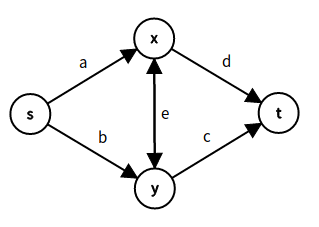
\includegraphics[width=2cm]  {graph1.png}}
  \end{figure}

  不再原来那几个方程?

  不过我们这里需要改变一下,我们将原本的多元关系转化一下,多设一个状态表示相邻的四个人是否选择文科或理科。

  这里以文科举例。

  记$x$为某个奇\;\male \;怪的同学,S集合表示选择文科,T集合表示理科,$y$表示是否需要都选择理科的加成(划到S集合表示放弃,划到T集合表示需要)。

  记文科收益为$a_x$,理科收益为$b_x$,额外的文科收益为$A_x$,额外的理科收益为$B_x$。
  
  那么我们就可以列出方程啦

  \begin{eqnarray*} 
    a + b &=&  a_x \\
    c + d &=&  b_x+B_x\\
    a + c + f &=& a_x+B_x\\
    b + d + e &=& inf\\
  \end{eqnarray*}
  特别地,如果发生冲突的话,即方程右边为$inf$

  解一解方程,得到
  
  \begin{eqnarray*} 
    a &=& a_x\\
    b &=& 0\\
    c &=& B_x\\
    d &=& b_x\\
    e &=& inf\\
    f &=& 0
  \end{eqnarray*}

  特别地,如果某个未知数的解为$0$直接忽略即可。
  
  对于文科加成,类似的解方程即可。

  那么我们就得到了建图方式

  \begin{itemize}
  \item 对于每一个人$i$,从源点连容量为$a_i$的边,连到汇点容量为$b_i$的边。
  \item 新建节点,表示额外的理科收益,连到汇点容量为$B_i$,将所有相邻的点以及自己连接到该点,容量为$inf$。
  \item 新建节点,表示额外的文科收益,从源点连边容量为$A_i$,同时连到所有相邻以及自己的点,容量为$inf$。
  \end{itemize}

  最终答案为$$\sum_{i,j}(a_{i,j}+b_{i,j}+A_{i,j}+B_{i,j})-minimalcut$$
  \newpage

  \section{长郡集训Day4-gift}
  \subsection{题目大意}
  给出$n$种物品,每种物品有$a_i$的花费。

  现在给出$m$种三元组关系$(p_i,q_i,b_i)$,表示同时购买$p_i,q_i$将获得收益$b_i$。

  设$A=\sum a_i,B=\sum b_i$。

  求最大化的$\frac{B}{A}$
  
  \subsection{数据范围}
  $1\le n \le 4000,1\le m \le 2\times 10^5$
  \subsection{思路}
  考虑最原始的建边,对于每一个物品连到汇点容量为$a_i$,对于每一种三元组,新建节点,源点连该节点容量为$b_i$,再从该点连到两个物品容量为$inf$,$65pts$。

  考虑优化,我们要求的是一个点集内部边权和的最大值,参考$Amber$的论文。

  记$deg_i$为$i$所连的边的权值和,即$\sum_{v\in S}w_{i,v}$

  $$\frac{B}{A} = \displaystyle\frac{\sum\displaystyle_{i\in S'}deg_i-cut[S',\bar S']}{2\sum\displaystyle_{i\in S'}a_i}$$

  分数规划,得

  $$\sum_{i\in S'}deg_i-cut[S',\bar S']> 2g\sum_{i\in S'}a_i$$

  $$\sum_{i\in S'}(deg_i-2ga_i)-cut[S',\bar S'] > 0$$

  我们要求上式的最大值,左右同乘$-1$,再加上极大数$U$。

  $$\sum_{i\in S'}(2ga_i-deg_i+U)+cur[S',\bar S'] < 0$$

  所以,我们可以运用最小割求解。

  从源点连接$U$的边到$i$,从$i$连边到$t$容量为$2ga_i-deg_i+U$。

  对于三元组,我们将$p_i,q_i$连接双向边,容量为$b_i$。

  跑最小割,判断是否有$$dinic()-nU<0$$

  \newpage

  \section{Codeforces808F-Card Game}
  \subsection{题目大意}
  给出$n$种物品,每种物品有三种属性,价值$c_i$,键值$p_i$,等级$l_i$。

  定义等级为$level$,无法选择$l_i>level$的物品。

  求最小的等级$level$,使得可以选出价值之和超过$k$的物品。

  注意,要求选出的物品中,任何两物品的价值之和不为质数。
  
  \subsection{数据范围}
  $1\le n \le 100$
  \subsection{思路}
  先二分等级$level$。
  
  比较明显的二分图,奇数放左边,偶数放右边,最后只需要求一次最大点权独立集。

  但是需要注意的是,$1+1=2$,$2$也是质数,所以我们需要特判完所有的$1$,选择价值最大的一个即可。
  
  \newpage

  \section{Tencent}
  \subsection{题目大意}
  给出$n$个人,其中有$m$对人如果同时选择会产生战斗力$w_i$。

  其中某些人是必须被选择的。

  记选出$k$个人,要求最大化$$\frac{\sum_{e\in E'}w_e}{k(2n-k)}$$
  
  \subsection{数据范围}
  $1\le n \le 400,1\le m\le min(10^5, n(n-1)/2)$
  \subsection{思路}
  最大密度子图,先推公式。

  分数规划$g$,得到

  $$\sum_{e\in E'}w_e-g\times k(2n-k)>0$$

  除以$2$,得到

  $$\sum_{e\in E'}\frac{w_e}{2}-kng+\frac{k^2g}{2} > 0$$
  
  继续拆开,变换形式,得

  $$\sum_{e\in E'}\frac{w_e}{2}+\frac{k(k-1)}{2}\times g-\sum_{v\in V'}(n-\frac{1}{2})kg >0$$

  同时乘上$-2$,得

  $$\sum_{v\in V'}(2n-1)g-\left[\frac{k(k-1)}{2}\times 2g+\sum_{e\in E'}w_e\right] < 0$$

  记$$\sum_{e\in E'}w'_e= \frac{k(k-1)}{2}\times 2g+\sum_{e\in E'}w_e$$

  由于$\frac{k(k-1)}{2}\times 2g$的形式是,一张有$k$个节点的完全图,所有边的权值均为$2g$,现在单独考虑$2g$的最小割,为$$\frac{\sum_{v\in E'}d_v-cut[s',\bar s']}{2}$$

  再考虑$w_e$,我们重新定义$d_u=\sum\limits_{v\in V}(w_{u,v}+2g)$

  得到

  $$\sum_{e\in E'}w'_e=\frac{\sum\limits_{v\in V'}d_v-cut[s', \bar s']}{2}$$

  我们将每个点的权值加上$(2n-1)g+U$,每条边的权值加上$2g$,规定一下建图方式。

  \begin{itemize}
  \item 对于每一个节点,连接汇点,容量为$(2n-1)g+U$
  \item 如果该点必须选择,则与源点容量为$inf$,否则为$U$
  \item 对于原图中的每条边,建边,容量为$w_{u,v}+2g$
  \end{itemize}

  二分的时候,只需要判断是否有$nU-maxflow>0$
  \newpage

  \section{LibreOJ-餐巾计划}
  \subsection{题目大意}
  在$n$天中每天需要$r_i$块餐巾,有三种选择。

  \begin{itemize}
  \item 购买餐巾,每块费用为$P$
  \item 快洗,耗时$M$天,费用为$F$
  \item 慢洗,耗时$N$天,费用为$S$
  \end{itemize}

  求在满足每一天需求的情况下的最小总花费。
  
  \subsection{数据范围}
  $1\le n \le 1000$
  \subsection{思路}
  难点主要是在,要分开清洗和使用,也就是拆点成两个表示今天送洗和使用的,知道这个后建图就容易了。

  记今天送洗的点为$x_i$,今天使用的点为$x_i'$。
  
  \begin{itemize}
  \item $s$连接$x_i$容量为$r_i$,花费为$0$
  \item $s$连接$x_i'$容量为$r_i$,花费为$P$
  \item $x_i'$连接$t$容量为$r_i$,花费为$0$
  \item $x_i$连接到$x_{i+1}$,容量为$inf$,花费为$0$
  \item $x_i$连接到$x_{i+N}'$容量为$inf$,花费为$S$
  \item $x_i$连接到$x_{i+M}'$容量为$inf$,花费为$F$
  \end{itemize}
  
  以上分别对应着三种情况,跑费用流。
    
  \newpage

  \section{LibreOJ-最长$k$可重区间集}
  \subsection{题目大意}
  给出$n$个区间,要求在满足任意数$x$被区间覆盖次数小与等于$k$的情况下的,区间总长度最长。

  求最长总长度。
  
  \subsection{数据范围}
  $1\le n \le 100$
  \subsection{思路}
  并没有发现是$k$条不相交路径的情况。

  知道之后的话,就好办了,每个区间看作点,拆点限流,排序后向不相交的区间连边,跑最大费用最大流。
    
  \newpage

  \section{BZOJ3144-切糕}
  \subsection{题目大意}
  给出$p\times q\times r$的长方体点阵,每个点有权值$v_{i,j,k}$。

  要求在$p\times q$个纵轴中,每个纵轴选一个点,同时满足相邻纵轴所选点的高度差不超过$D$。

  现在需要求出最小的$\sum\limits_{(i,j,k)\in S} v_{i,j,k}$。
  
  %{\setmainfont{Lato-LightItalic}  1234asdklsdnfklasdnfklasd Ubuntu}  
  %\setmainfont{原来的字体}
    
  \subsection{数据范围}
  $1\le p,q,r \le 40$
  \subsection{思路}
  弄张图出来
  
  \begin{figure}[htb]
    \center{\includegraphics[width=2.5cm]  {graph3.png}}
  \end{figure}
  
  这种模型叫做伟大的距离限制模型。

  现在不同于二元组模型,现在将点权下放到边,然后割掉哪一条边表示选择哪一个点。

  \newpage
  
  现在来考虑限制,只考虑一条链的情况,我们应该这样连边。
  
  \begin{figure}[htb]
    \center{\includegraphics[width=2.5cm]  {graph4.png}}
  \end{figure}

  非常奇怪的图,现在假设我们选择了$(2,3)$之间的边,割掉之后,由于有$(2,4)$这条$inf$边的限制,我们只能选择$4$下面的边割掉,同时限制是双向的,也就达到了只能选择$[k-D,k+D]$的限制。

  然后就是最小割

  \newpage

  \section{TopCoder-Fox And City}
  \subsection{题目大意}
  给出一张$n$个点,$m$条边的有向无环图,边权均为单位距离,顶点标号从$1-n$。

  现在你可以有任意次在任意两点之间加边。
  
  定义加完所有边之后,$d_i$为点$i$到点$1$的距离,每个节点有期望距离$w_i$。

  要求你最小化$$\sum_{i=2}^n(d_i-w_i)^2$$
  
  %{\setmainfont{Lato-LightItalic}  1234asdklsdnfklasdnfklasd Ubuntu}  
  %\setmainfont{原来的字体}
    
  \subsection{数据范围}
  $1\le n \le 40$
  \subsection{思路}
  首先要知道几个性质:

  \begin{itemize}
  \item 有且仅有$d_1 = 0$
  \item 若存在边$(u,v)$,则存在$|d_u-d_v| \le 1$
  \item 若存在$d_i=k$,则一定存在$j$,有$d_j=k-1$
  \item 对于所有$i$,有$d_i< n$
  \end{itemize}

  考虑上面的性质,也就是所有的$d_i(i \not = 1)$必须在$[1,n-1]$之间选择。

  如果有两点之间有边,那么就会存在限制,距离限制模型。

  现在考虑建边,记$P_{i,j}$表示点$i$选择的数小于等于$j$。

  那么,我们将每一点拆成一串数$P_{i,0},P_{i,1},P_{i,2},...,P_{i,n-1}$。(距离限制模型的建法)

  首先因为$d_1=0$,所以我们要强制选择$P_{i,0}$。

  然后对于$i(i \not = 1)$,将点权下放到边权上,边权为代价。

  这里可以用最小割的模型来解释,与$S$相连的点为$False$,与$T$相连的点为$True$,割掉一条,其两边的点是符合解释的。

  根据距离限制模型,我们对于已经存在的边$(u,v)$,连接边$(P_{u,k},P_{v,k-1}),(P_{v,k},P_{u,k-1})\;\;(k\in [2,n-1])$,对应着限制2。

  然后跑最小割即可。
  
  \newpage

  \section{BZOJ2229-ZJOI11最小割}
  \subsection{题目大意}
  给出$n$个点$m$条边的无向图。

  多组询问,询问图中所有点对的最小割满足最小割小于等于$x$的对数。
  
  %{\setmainfont{Lato-LightItalic}  1234asdklsdnfklasdnfklasd Ubuntu}  
  %\setmainfont{原来的字体}
    
  \subsection{数据范围}
  $1\le n \le 150$
  \subsection{思路}
  首先分治+最小割。

  在分治的过程中,更新答案,因为跑一次最小割将图分成了两个点集,所以我们将所有不在同一集合的点对更新一下最小割即可。
  
  \newpage

  \section{BZOJ3171-TJOI11循环格}
  \subsection{题目大意}
  给出$n\times m$的网格,网格上有箭头,到达某点会继续往箭头方向前进。

  现在求最小的修改次数,使得从任意点出发能够走回来。
  
  %{\setmainfont{Lato-LightItalic}  1234asdklsdnfklasdnfklasd Ubuntu}  
  %\setmainfont{原来的字体}
    
  \subsection{数据范围}
  $1\le n \le 25$
  \subsection{思路}
  首先,每个点的出入度都只能为$1$,想到了二分图。

  不过这里是带权二分图匹配,因为要跑费用流(在满足最大流的情况下跑花费小的),所以我们交换一下$AB$部。

  将$A$部看做点的出度,$B$部看做点的入度,对于一个点向原来的方向连接费用为$0$,否则连接费用为$1$的边。

  跑最小费用流。
  
  \newpage

  \section{BZOJ3442-学习小组}
  \subsection{题目大意}
  给出$m$种学习小组,每个学习小组报名费用为$f_i$,给出$n$个学生,每个学生最多参与$k$个学习小组,以及是否愿意参加某个学习小组。

  若有$a$个人参加第$i$个学习小组,将会产生$c_i\times a^2$的支出。

  要求在满足每个学生都参与的情况下,最小化\;支出-收入。
  
  %{\setmainfont{Lato-LightItalic}  1234asdklsdnfklasdnfklasd Ubuntu}  
  %\setmainfont{原来的字体}
    
  \subsection{数据范围}
  $1\le n \le 100$
  \subsection{思路}
  考虑平方的费用如何处理,这个可视作与流量有关的费用函数,由于费用流会优先选择费用小的,只需要把平方拆开,每条边的费用为$2\times (i-1)+1$(满足和为平方)即可。

  由于要满足每个学生都参与,所以考虑这样连边。

  从源点连到学生流量为$1$,学生连到汇点容量为$k-1$(满足至少参加一个)。

  学生连到学习小组,费用为$-f_i$,学习小组有$n$条边连到汇点,其中第$i$条边费用为$2\times (i-1)+1$。

  \newpage

  \section{BZOJ4205-卡牌配对}
  \subsection{题目大意}
  给出$n_1$种$x$类卡牌,$n_2$种$y$类卡牌,每张卡牌分别有属性$A_i,B_i,C_i$。

  两张卡牌能够配对,当且仅当,最多有一项属性值互质。

  求最大匹配数量。
  
  %{\setmainfont{Lato-LightItalic}  1234asdklsdnfklasdnfklasd Ubuntu}  
  %\setmainfont{原来的字体}
    
  \subsection{数据范围}
  $1\le n_1,n_2 \le 30000,1\le A_i,B_i,C_i\le 200$
  \subsection{思路}
  肯定是不能暴力连边的。

  发现$A_i,B_i,C_i\le 200$,考虑优化连边。

  最多有一项属性互质,那么至少有两项属性不互质,从这里入手,将所有有某种共同限制的点连接到一个点上。

  记$(x,y,z,k)$,表示属性$x_i$的质因子有$z$,属性$y_i$的质因子有$k$。

  继续考虑点的数量,由于在$[1,200]$以内的质数只有$46$个,所以我们只增加了$3\times 46\times 46$个点。

  考虑边,有$60000$个点,每个点最多可以连接$3\times 3\times3$条边,所以有$2000000$条边。

  虽然看起来还是比较暴力...

  我们把$n_1,n_2$作为二分图的$A,B$部,分别向新建的点连边,做二分图匹配。
  
  \newpage

  \section{BZOJ1283-序列}
  \subsection{题目大意}
  给出长度为$n$的序列$\{C_n\}$。

  要求选出一些数满足任意长度为$m$的连续子区间中选出的数不超过$k$个,求最大和。
  
  
  %{\setmainfont{Lato-LightItalic}  1234asdklsdnfklasdnfklasd Ubuntu}  
  %\setmainfont{原来的字体}
    
  \subsection{数据范围}
  $1\le n_1 \le 1000$
  \subsection{思路}
  构图挺巧妙的。

  考虑将问题转化一下,问题是选出$k$个数,我们考虑选出区间,也就是我们选出一个数相当于其包含的所有区间都被选择了一次。

  考虑这样构图,将序列用容量为$k$,费用为$0$的边串起来,再将点$i$连到点$i+m$容量为$1$费用为$C_i$。

  考虑正确性,对于一个点$i$,如果我们选择了它,那么包含$i$的所有区间的选择次数就减少了$1$,就是流量减少$1$,再通过边的流量限制,达到了$k$的限制。
  
  \newpage

  \section{BZOJ1449-球队收益}
  \subsection{题目大意}
  现在有$n$支球队,每只球队已经赢了$w_i$场,输了$l_i$场比赛,同时每只球队有收益系数$C_i,D_i$。

  设某球队最后赢了$x$场,输了$y$场,最后获得收益$C_i\times x^2+D_I\times y^2$。

  现在还剩下$m$场比赛,在任意决定比赛胜负的情况下,求收益总和的最小值。

  %{\setmainfont{Lato-LightItalic}  1234asdklsdnfklasdnfklasd Ubuntu}  
  %\setmainfont{原来的字体}
    
  \subsection{数据范围}
  $1\le n \le 5000$
  \subsection{思路}
  考虑一种实现起来非常复杂的方法。
  
  即对于每支队伍拆成两个点,分别表示队伍或者输(\sout{正确性无法保证})。
  
  考虑增量将收益拆开,先假设对于队伍$x$,尚未参加的比赛全输,考虑每赢一场的贡献。

  记$d_i$为剩下比赛中$x$队伍参与的场数。
  
  赢$0$场,收益为$C_i\times w_i^2+D_i(l_i+d_i)^2$

  赢$1$场,收益为$C_i\times (w_i+1)^2+D_i(l_i+d_i-1)^2$

  赢$2$场,收益为$C_i\times (w_i+2)^2+D_i(l_i+d_i-2)^2$

  赢$d_i$场,收益为$C_i\times (w_i+d_i)^2+D_i\times l_i$

  差分一下,发现收益是一个下凸函数

  赢$j$的收益为$C_i[2w_i+(2j-1)]-D_i[2(l_i+d_i)-(2j-1)] $
  
  把收益拆边即可。
  
  \newpage

  \section{BZOJ2879-美食节}
  \subsection{题目大意}
  现在有$n$个菜品,$m$个厨师,第$j$个厨师制作第$i$个菜品的时间为$t_{i,j}$。

  现在每道菜的需求为$p_i$,合理安排,求最小总等待时间。

  %{\setmainfont{Lato-LightItalic}  1234asdklsdnfklasdnfklasd Ubuntu}  
  %\setmainfont{原来的字体}
    
  \subsection{数据范围}
  $1\le n \le 40,1\le m\le 100$
  \subsection{思路}
  修车加强版,放在一起写了。

  考虑每一个菜的贡献,从当前这道菜到最后一道的数量记为$k$,那么其贡献为$k\times t_{i,j}$。

  从这个思路出发,我们将厨师拆成$\sum p_i$个,表示该厨师倒数第$i$次做的菜,时间为$i\times t_{i,j}$。

  估算一下点数边数,有点虚,继续优化,发现并不是所有的厨师都做了$\sum p_i$个菜,所有我们动态加边,也就是当前增广的厨师做的是倒数第$k$个菜,我们就再给该厨师连上$k+1$次的所有菜。
  
  \newpage

  \section{BZOJ4514-数字配对}
  \subsection{题目大意}
  给出$n$个三元组$(a_i,b_i,c_i)$。
  若第$i,j$个三元组,满足$a_i$是$a_j$的倍数,且$a_i/a_j$是质数,那么可以配对并获得$c_i\times c_j$的价值。

  要求在总价值不小于$0$的前提下,求最多进行的配对次数。
  
  %{\setmainfont{Lato-LightItalic}  1234asdklsdnfklasdnfklasd Ubuntu}  
  %\setmainfont{原来的字体}
    
  \subsection{数据范围}
  $1\le n \le 200$
  \subsection{思路}
  若$a_i/a_j$是质数,那么其质因数的个数肯定是一奇一偶,我们可以根据这个做二分图。

  奇数放左边,偶数放右边,能配对的连接。

  一直跑最大费用流,直到价值小于$0$,总流量为答案。
  \newpage

  \section{BZOJ1001-狼抓兔子}
  \subsection{题目大意}
  给出$n\times m$的网格,给出横向纵向斜向的道路,每条边有边权$w_i$。

  求将$(1,1)$与$(n,m)$分隔开的最小代价。
  
  %{\setmainfont{Lato-LightItalic}  1234asdklsdnfklasdnfklasd Ubuntu}  
  %\setmainfont{原来的字体}
    
  \subsection{数据范围}
  $1\le n,m \le 1000$
  \subsection{思路}
  直接利用最小割的定义建图,然而边数太多,只能优化。

  考虑优化,这是一张平面图,将每个小三角形视为点,我们的割就是一条路径将这些点连接。

  就是我们求出的最小割连接起来就是一条将网格分开的曲线,按照这个跑最短路即可。
  \newpage

  \section{BZOJ1061-志愿者招募}
  \subsection{题目大意}
  给出$n$天,每天有需求$a_i$,有$m$种志愿者,第$i$种志愿者可以在$[s_i,t_i]$工作,每人费用为$c_i$。

  求满足要求的最小费用。
  
  %{\setmainfont{Lato-LightItalic}  1234asdklsdnfklasdnfklasd Ubuntu}  
  %\setmainfont{原来的字体}
    
  \subsection{数据范围}
  $1\le n \le 1000,1\le m\le 10000$
  \subsection{思路}
  根据姜志豪的论文,我们可以这样考虑。

  先从特殊情况考虑,现在假设有$3$种志愿者,记$(x,y,z)$为区间为$[x,y]$,费用为$z$。

  已知$([1,3],c_1),([2,3],c_2),([1,2],c_3)$

  记$p_i$表示$i$天总共招募的人,$b_i$表示第$i$种志愿者招募的数量。

  得到不等式:

  \begin{eqnarray*} 
    p_1=b_1+b_3 &\ge& a_1 \\
    p_2=b_1+b_2+b_3 &\ge& a_2 \\
    p_3=b_1+b_2 &\ge& a_3
  \end{eqnarray*}

  记$d_i$为补偿量,转成等式,相邻两等式做差,得到:

  \begin{eqnarray*} 
    p_1 = b_1+b_3-d_1 &=& a_1 \\
    p_2-p_1 = b_2+d_1-d_2 &=& a_2-a_1 \\
    p_3-p_2 = -b_3+d_2-d_3 &=& a_3-a_2 \\
    -p_3 = -b_1-b_2 &=& -a_3-d_3 
  \end{eqnarray*}

  注意等式的形式,最左边我们构造成这样,右边为常数项。

  对于数$x$,若$x$为正,我们认为它需要流出,$x$为负,我们认为它需要流入。

  上述等式应该满足流量平衡,我们将第$i$个等式视作网络中的第$i$个点,那么得到了$n+1$个点,同时添加源汇点$s,t$。
  
  同时对于变量$x$,若它在第$i$个等式中为正,第$j$个等式中为负,我们则将$(i,j)$连接。

  对于常数$a_i-a_{i-1}$,若为正,则源点向其连边,若为负,则向汇点连边。
  
  同时对于变量$b_i$,我们应该将它的费用设置为$c_i$。

  \newpage
  
  综合一下:

  \begin{itemize}
  \item 对于常数$a_i-a_{i-1}$,若为正,则源点向其连边容量为$a_i-a_{i-1}$,若为负,则向汇点连边容量为$a_{i-1}-a_i$。
  \item 对于$b_i$,我们连边$(s_i,t_i)$,容量为$inf$,费用为$c_i$。
  \item 对于$d_i$,我们连边$(i,i-1)$,容量为$inf$,费用为$0$。
  \end{itemize} 
  \newpage

  \section{BZOJ3112-防守战线}
  \subsection{题目大意}
  给出长度为$n$的序列,在点$i$建造塔的费用为$c_i$,可以在一个位置建造任意多的塔。

  现在给出$m$个区间,$[L_i,R_i]$,要求在$[L_i,R_i]$区间内至少有$D_i$座塔。

  求满足要求的最小费用。
  
  %{\setmainfont{Lato-LightItalic}  1234asdklsdnfklasdnfklasd Ubuntu}  
  %\setmainfont{原来的字体}
    
  \subsection{数据范围}
  $1\le n \le 1000,1\le m\le 10000$
  \subsection{思路}

  记$x_i$表示$i$点建造塔的数量。
  
  我们要求最小化$\sum\limits_{i=1}^n C_ix_i$

  列出限制条件
  
  \begin{eqnarray*} 
    \sum_{i=L_1}^{R_1}x_i \ge D_1 \\
    \sum_{i=L_2}^{R_2}x_i \ge D_2\\
    ~\\
    ...\\
    \sum_{i=L_m}^{R_m}x_i \ge D_m
  \end{eqnarray*}

  弄个特殊点出来手玩

  要求最小化$C_1x_1+C_2x_2+C_3x_3$
  
  \begin{eqnarray*} 
    x_1+x_2+x_3 \ge D_1 \\
    x_2+x_3 \ge D_2\\
    x_1+x_2 \ge D_3
  \end{eqnarray*}

  \newpage

  把系数放到系数矩阵中,第一行放收益系数$C_i$,第一列放限制$D_i$

  
  \begin{tabular}{c|ccc}
    \hline 0&$C_1$&$C_2$&$C_3$\\
	\hline $D_1$&1&1&1\\
	\hline $D_2$&0&1&1\\
	\hline $D_3$&1&1&0\\
	\hline
  \end{tabular}

  ~\\
  
  转置一下

  ~\\
  
  \begin{tabular}{c|ccc}
    \hline 0&$D_1$&$D_2$&$D_3$\\
	\hline $C_1$&1&0&1\\
	\hline $C_2$&1&1&1\\
	\hline $C_3$&1&1&0\\
	\hline
  \end{tabular}

  ~\\
  
  得到了其对偶问题

  要求最大化$D_1x_1+D_2x_2+D_3x_3$
  
  \begin{eqnarray*} 
    x_1+x_3 &\le& C_1 \\
    x_1+x_2+x_3 &\le& C_2\\
    x_1+x_2 &\le& C_3
  \end{eqnarray*}

  按照志愿者招募的套路,得到方程组

  \begin{eqnarray*} 
    x_1+x_3+d_1 &=& C_1 \\
    x_2+d_2-d_1 &=& C_2-C_1\\
    -x_3+d_3-d_2+ &=& C_3-C_2\\
    -x_1-x_2-d_3 &=& -C_3
  \end{eqnarray*}

  正的表示需要流出,负的表示需要流入,连边跑费用流。

  \sout{卡SPFA}
  
  \newpage

  \section{BZOJ1927-星际竞速}
  \subsection{题目大意}
  给出$n$个点,你可以从初始点跳到$i$点,费用为$w_i$(只能跳一次)。

  现在给出边$(u,v,c)$,从编号小的点$u$,到编号大的点$v$,费用为$c$。

  求遍历所有点的最小费用。
  
  %{\setmainfont{Lato-LightItalic}  1234asdklsdnfklasdnfklasd Ubuntu}  
  %\setmainfont{原来的字体}
    
  \subsection{数据范围}
  $1\le n \le 1000$
  \subsection{思路}

  \sout{明明就是与餐巾计划一样}。

  拆点费用流,一个表示出点,一个表示入点。

  \begin{itemize}
  \item 将入点连到汇点,容量为$1$,费用为$0$,将源点与每个出点连接费用为$0$。
  \item 将源点与每个入点连接费用为$w_i$。
  \item 对于每一条边,将$u$的出点与$v$的入点连边,容量为$1$,费用为$c$。
  \end{itemize}

  对于这种问题,最大流可能会应为费用的问题达不到我们想要的效果,所以,我们通过拆点,强行加上某些边。
  
  \newpage

  \section{Vijos1891-学姐的逛街计划}
  \subsection{题目大意}
  给出$3\times n$个点,每个点有权值$a_i$,要求从中选出一些点,并且在满足任意连续的$n$个数中不得选超过$k$个数。

  求选出的最大权值。
  
  %{\setmainfont{Lato-LightItalic}  1234asdklsdnfklasdnfklasd Ubuntu}  
  %\setmainfont{原来的字体}
    
  \subsection{数据范围}
  $1\le n \le 1000$
  \subsection{思路}

  线性规划,日常列式子。

  记$x_i$为第$i$天的决定,为$0$表示不选,为$1$表示选。

  要求最大化$\sum\limits_{i=1}^{3\times n}a_ix_i$

  现在假设$n=3$。
  
  \begin{eqnarray*} 
    x_1+x_2+x_3 &\le& k \\
    x_2+x_3+x_4 &\le& k \\
    x_3+x_4+x_5 &\le& k \\
    ...
    ~\\
    x_7+x_8+x_9 &\le& k
  \end{eqnarray*}

  按照志愿者招募的套路,记$d_i$为第$i$个式子的补偿量,做差得到。

  \begin{eqnarray*} 
    x_1+x_2+x_3+d_1 &=& k \\
    x_4-x_1+d_2-d_1 &=& 0 \\
    x_5-x_2+d_3-d_2 &=& 0 \\
    ...
    ~\\
    -x_7-x_8-x_9-d_7 &=& -k
  \end{eqnarray*}

  \begin{itemize}
  \item 从源点连到点$1$,从点$3\times n-1$到源点都连接容量为$k$的费用为$0$的边
  \item 从点$i$连到点$i+1$容量为$inf$费用为$0$的边
  \item 根据$x_i$的出现连接相应的点
  \end{itemize}
  
  \newpage

  \section{BZOJ1930-Pacman 吃豆豆}
  \subsection{题目大意}
  给出$n$个豆豆,每个豆豆的坐标为$(x_i,y_i)$。

  要求两个$Pacman$可以向上或者向右走,在路线不相交的情况下求最多能吃掉的豆豆。
  
  %{\setmainfont{Lato-LightItalic}  1234asdklsdnfklasdnfklasd Ubuntu}  
  %\setmainfont{原来的字体}
    
  \subsection{数据范围}
  $1\le n \le 1000$
  \subsection{思路}

  首先,路线不相交的情况是可以调整一下顺序去掉的,也就是说这个条件没有用。

  然后暴力连边,发现有$n^2$条边,并不可行。

  优化一下连边,对于点$i,j,k$,如果$i,j$与$j,k$互达,那么$(i,k)$的边可以不连。

  但是会出现一种情况,原本不会经过点$i$两次,但是在点$i$处相交了,就会损失$1$的流量,所以需要将流量设置为$2$。
  
  \newpage

  \section{BZOJ2597-WC07剪刀石头布}
  \subsection{题目大意}
  给出一张竞赛图,其中某些边的方向未确定,求任意安排边的方向使得出现的三元环最多。
  
  %{\setmainfont{Lato-LightItalic}  1234asdklsdnfklasdnfklasd Ubuntu}  
  %\setmainfont{原来的字体}
    
  \subsection{数据范围}
  $1\le n \le 100$
  \subsection{思路}

  首先,我们可以通过补集的思想考虑问题。

  在任意三点中,如果某个点的出度大于等于$2$,那么这就不是一个合法的三元环。

  那么问题就转化为求$C_n^3-\sum\limits_{i=1}^nC_{deg_i}^2$。

  由于$C_n^3$已知,所以我们要求$\sum\limits_{i=1}^nC_{deg_i}^2$的最小值。

  到这里问题就可以用费用流来做了,我们将所有的比赛看作点。

  我们规定一下若存在边$(x,y)$表示$x$胜了$y$。
  
  \begin{itemize}
  \item 若在$i,j$中已经有了胜负,则向赢的人连边容量为$1$费用为$0$
  \item 若在$i,j$中尚未决出胜负,则向两人连边
  \item 每个人向汇点连边,将组合数拆边为贡献
  \end{itemize}
  
  跑最小费用流。
  \newpage

  \section{BZOJ2406-矩阵}
  \subsection{题目大意}
  给出矩阵$A_{n,m}$,求出矩阵$B_{n,m}$,满足$\forall 1\le i\le n,1\le j\le m,B_{i,j}\in[L,R]$

  求下式的最小值

  \[max\left\{\begin{array}{ll}
  \max\limits_{1\le j \le m}\left\{|\sum\limits_{i=1}^n(A_{i,j}-B_{i,j})|\right\}&\\
  ~\\
  \max\limits_{1\le i\le n}\left\{|\sum\limits_{j=1}^m(A_{i,j}-B_{i,j})|\right\}&
  \end{array}\right.\]
  
  %{\setmainfont{Lato-LightItalic}  1234asdklsdnfklasdnfklasd Ubuntu}  
  %\setmainfont{原来的字体}
    
  \subsection{数据范围}
  $1\le n \le 100$
  \subsection{思路}
  
  最大值最小,二分一下答案,记为$mid$。

  那么对于每一行每一列我们都可以得到下式

  $$| \sum A_{i,j}-\sum B_{i,j}| \le mid$$

  变一变,得到

  $$\sum A_{i,j}-mid\le B_{i,j}\le \sum B_{i,j}+mid$$

  \sout{现在就是一个有源汇的上下界的模板题啦}

  将行列作为二分图的$A,B$部,每一行向每一列连接上下界为$[L,R]$的边,

  $S$向每一行,每一列向$t$连接上下界为$[\sum A_{i,j}-mid,\sum A_{i,j}+mid]$

  按照有源汇的上下界流处理
  \newpage

  \section{BZOJ2560-串珠子}
  \subsection{题目大意}
  给出$n$个点,第$i,j$个点之间有$C_{i,j}$条边可以连接。

  求所有点联通的方案数。
  
  %{\setmainfont{Lato-LightItalic}  1234asdklsdnfklasdnfklasd Ubuntu}  
  %\setmainfont{原来的字体}
  
  \subsection{数据范围}
  $1\le n \le 16$
  \subsection{思路}
  考虑补集转化,即所有方案减去不合法的方案。

  现在考虑处理出集合$s$任意连接的方案,记$f_{s}$为$s$集合任意连接的方案数,那么我们可以得到方程

  $$f_{s}=\prod_{i,j\in s} C_{i,j}$$

  记$g_s$表示$s$集合得到的合法方案,那么我们可以得到方程

  $$g_s=f_s-\sum_{s'\subset s}(g_{s'}\times f_{\bar s})$$

  为了不重不漏,我们可以枚举每一个状态最后一个$1$的位置(记为$j$),分成两个集合,包含$j$的,不包含$j$的,那么就是$g_{(p|j \subset p)}\times f_{(q|j \not\subset q)}$
  \newpage

  \subsection{题目大意}
  给出$n$家商店,给出$m$件商品。

  到达第$i$家的商店路费为$d_i$,在第$i$家商店购买第$j$种商品的费用为$c_{i,j}$。
  
  %{\setmainfont{Lato-LightItalic}  1234asdklsdnfklasdnfklasd Ubuntu}  
  %\setmainfont{原来的字体}
  
  \subsection{数据范围}
  $1\le n \le 16,1\le m\le 100$
  \subsection{思路}
  记$f_{i,s}$为当前枚举到第$i$家商店,已经购买$s$集合的商品。
  
  有一个显然的思路$n\times 3^m$(枚举子集),也是显然T。

  如果我们到达商店$i$却不购买任何东西,这样是不会更优的。

  根据这个,我们可以强行令$f_{i,j}=f_{i-1,j}+d_i$。

  记$j$为当前集合,$k$为待购买的物品,$s'$为购买之后的集合。
  
  然后枚举购买的物品,即

  $$f_{i,s'}= min\{f_{i,s | k \not\subset s} + c_{i,k}\}$$

  如果我们不购买物品,再将$f_{i,j}$更新回去,即

  $$f_{i,j}=min\{f_{i,j},f_{i-1,j}\}$$
  \newpage

  \section{Walk}
  \subsection{题目大意}
  给出$n$个点,$m$条无向边,每个节点有权值$a_i$。

  若从$i$走到相邻的点$j$,需要满足$a_i>a_j$。

  但你有$k$次机会不遵守上述约定,求最多能到达的点的个数。
  %{\setmainfont{Lato-LightItalic}  1234asdklsdnfklasdnfklasd Ubuntu}  
  %\setmainfont{原来的字体}
  
  \subsection{数据范围}
  $1\le n \le 10^5,1\le m\le 2\times 10^5$
  \subsection{思路}
  记$f_{i,j}$表示到达点$i$已经使用了$j$次机会的最多到达的点。

  转移是显然的,然而会存在后效性。

  我们考虑将能直接走的点分层一下,变成单独的图,这张图是不存在环的,为了消除后效性,我们需要将$i$所有能够直接到达的点放在$i$的前面更新。

  直接拓扑排序,于是有方程:

  $$f_{i,j}=\max_{a_k<a_i}f_{k,j}+1$$

  $$f_{i,j}=\max_{a_k \ge a_i}f_{k,j-1}+1$$

  为了卡空间,滚动数组优化一下。
  
  \newpage

  \section{Ticket}
  \subsection{题目大意}
  给出$m$个$s$,$n$个$x$。

  现在任意排列$n+m$个字母,要求在满足在任意位置$s$的个数大于$x$的个数,求合法方案数。
  %{\setmainfont{Lato-LightItalic}  1234asdklsdnfklasdnfklasd Ubuntu}  
  %\setmainfont{原来的字体}
  
  \subsection{数据范围}
  $1\le n,m \le 5\times 10^3$
  \subsection{思路}

  \begin{figure}[htb]
    \center{\includegraphics[width=5.6cm]  {graph5.png}}
  \end{figure}
  
  在二维平面上画出$y=x$的图像,记向右走为使用一个$s$,向上走为使用一个$t$。

  那么,合法方案是不允许超过$y=x$直线到达$(m,n)$的方案数。

  从$(0,0)$出发到达$(m,n)$的方案数(不考虑是否合法)为$C_{n+m}^n$。

  现在暂不考虑允许在$y=x$直线上的情况,考虑一一对应。

  合法方案肯定第一步走到$(1,0)$,而不合法方案第一步位于$(0,1)$。

  从$(0,1)$走在$(m,n)$的方案沿直线$y=x$翻折后唯一对应着一种不合法方案。

  现在考虑允许在$y=x$直线上的情况,即将直线$y=x$上移,变成$y=x+1$。

  出发点是$(0,0)$,翻折后是$(-1,1)$,所有方案数为$C_{n+m}^m$。

  从$(-1,1)$出发的方案数为$C_{n+m}^{m+1}$。

  所以方案数为$$\binom{n+m}{m}-\binom{n+m}{m+1}$$

  ~\\
  
  现在从另外一个角度考虑问题,对于有$m$个$s$,$n$个$x$的不合法串$sxsxsxx$,我们将它$sx$反转。

  得到了有$m+1$个$s$,$n-1$个$x$的串,可以证明这样的反转是一一对应的。

  那么可以知道不合法的方案是$\binom{m+n}{m+1}$。

  依旧可以得到方案数为$$\binom{n+m}{m}-\binom{n+m}{m+1}$$

  \section{BZOJ3036-绿豆蛙的归宿}
  \subsection{题目大意}
  给出$n$个点$m$条边长度为$w$的有向无环图,起点为$1$,终点为$n$。

  求从起点$1$到达点$n$的期望长度。
  %{\setmainfont{Lato-LightItalic}  1234asdklsdnfklasdnfklasd Ubuntu}  
  %\setmainfont{原来的字体}
  
  \subsection{数据范围}
  $1\le n,m \le 10^5$
  \subsection{思路}
  
  记$f_i$为点$i$到达点$n$的期望长度。

  根据全期望公式
  
  $$E(Y)=\sum P(x=x_i)\times E(Y|x=x_i)$$

  其中$E(Y|x=x_i)$表示$Y$事件在$x=x_i$事件发生后的期望。

  记$|G_i|$为点$i$到达的集合。

  那么有方程$$f_u=\sum_{v\in |G_i|} \frac{f_v+cost_{u,v}}{|G_i|}$$

  对于$f_v$,我们在$u$点选择的时候需要$\frac{1}{|G_i|}$的概率选择点$v$,所以我们在算期望的时候也需要乘上$\frac{1}{|G_i|}$
  \newpage

  \section{Codeforces518D-IIya and Escalator}
  \subsection{题目大意}
  现在有$n$个人排成一列,每秒队伍最前面的人有$p$的概率走上电梯(一旦上去将不会走下来),或者有$1-p$的概率不动,求$t$秒后,在电梯上的人的期望。
  
  %{\setmainfont{Lato-LightItalic}  1234asdklsdnfklasdnfklasd Ubuntu}  
  %\setmainfont{原来的字体}
  
  \subsection{数据范围}
  $1\le n,t \le 2\times 10^3, 0\le p\le 1$
  \subsection{思路}
  
  记$f_{i,j}$为第$i$秒电梯上有$j$人的概率(由于期望的线性性质,我们可以先算概率,最后求期望)。

  那么转移就非常的显然了。

  $$f_{i+1,j} \leftarrow f_{i,j}\times (1-p)$$
  $$f_{i+1,j+1} \leftarrow f_{i,j}\times p$$

  注意,若电梯上已经有了$n$个人,那么有$$f_{i+1,n}\leftarrow f_{i,n}$$。
  \newpage

  \section{BZOJ1419-Red is good}
  \subsection{题目大意}
  现在有$r$张红牌,$b$张黑牌,现在随机排列成一列。

  每翻开一张红牌得到$1$美元,翻开一张黑牌付出$1$美元,你可以随时停下来。

  求最优策略下收益的期望。
  
  %{\setmainfont{Lato-LightItalic}  1234asdklsdnfklasdnfklasd Ubuntu}  

  \subsection{数据范围}
  $1\le n,t \le 5\times 10^3$
  \subsection{思路}
  
  记$f_{i,j}$为剩下$i$张红牌,$j$张黑牌的期望。

  初始状态为$f_{0,0} = 0$。

  对于当前状态$(i,j)$,根据全期望公式,得到方程

  $$f_{i,j}=(f_{i-1,j}+1)\times \frac{i}{i+j}+(f_{i,j-1}-1)\times \frac{j}{i+j}$$

  同时还要求最优策略,那么如果期望为负,我们就会停下来,那么此时的期望为$0$。

  即

  $$f_{i,j}=max(0, (f_{i-1,j}+1)\times \frac{i}{i+j}+(f_{i,j-1}-1)\times \frac{j}{i+j})$$

  \newpage

  \section{BZOJ4350-Easy}
  \subsection{题目大意}
  给出长度为$n$的由$x,o,?$组成的字符串,其中$?$表示各有$50\%$的几率变成$x,o$。

  若存在连续的$a$个$o$,会得到积分$a^2$。

  求最后得分的期望。
  %{\setmainfont{Lato-LightItalic}  1234asdklsdnfklasdnfklasd Ubuntu}  

  \subsection{数据范围}
  $1\le n \le 3\times 10^5$
  \subsection{思路}
  
  记$f_i$表示前$i$个字符的得分期望,由于我们需要考虑连续的长度,所以我们还需要多记录$l_i$表示$i$位置结尾的连续的期望长度。

  得分是平方项(根据费用流,我们知道这个是可以拆开的),$(l_i+1)^2-l_i^2=2i+1$

  记$s_i$表示第$i$个字符。

  若$s_i=x$,则有$f_i=f_{i-1}\;\;\;\;\;l_i=0$

  若$s_i=o$,则有$f_i=f_{i-1}+2l_{i-1}+1\;\;\;\;\;l_i=l_{i-1}+1$

  若$s_i=?$,则有$f_i=f_{i-1}+\frac{2l_i+1}{2}\;\;\;\;\;l_i=\frac{l_{i-1}+1}{2}$
  \newpage

  \section{BZOJ4318-OSU!}
  \subsection{题目大意}
  现在长度为$n$的01串,每个位置$i$有$p_i$的几率为$1$。

  若存在连续的长度为$a$的$1$,将得到分数$a^3$。

  求得分的期望。
  %{\setmainfont{Lato-LightItalic}  1234asdklsdnfklasdnfklasd Ubuntu}  

  \subsection{数据范围}
  $1\le n \le 3\times 10^5$
  \subsection{思路}
  
  类似与上一题,我们考虑贡献,$(l_i+1)^3-l^3_i=3l_i^3+3l_i+1$。

  那么我们需要维护期望长度的平方以及期望长度即可。

  记$d_i$为$i$位置期望长度的平方,可以得到,$(l_{i-1}+1)^2=l_{i-1}^2+2l_{i-1}+1=d_{i-1}+2l_{i-1}+1$

  根据全期望公式,$E(Y)=\sum P(x=x_i)E(Y|x=x_i)$

  (注意$E(Y|x=x_i)$表示$x=x_i$事件发生后事件$Y$的期望)。

  记$f_i$表示在$i$位置的得分期望。
  
  得到$$f_i=f_{i-1}\times (1-p)+(f_{i-1}+3d_{i-1}+3l_{i-1}+1)\times p=f_{i-1}+p\times (3d_{i-1}+3l_{i-1}+1)$$

  注意,如果是抽中$0$,那么不会产生贡献,则$E(Y|x=x_i)=f_{i-1}$
  \newpage

  \section{COGS1489-玩纸牌}
  \subsection{题目大意}
  现在某个人有$p$的概率赢,$1-p$的概率输。

  如果某天胜率超过$p$则停止当天的游戏,但如果超过$n$盘依旧没有达到要求则停止所有的游戏。

  求他能够玩游戏的天数的期望。
  %{\setmainfont{Lato-LightItalic}  1234asdklsdnfklasdnfklasd Ubuntu}  

  \subsection{数据范围}
  $1\le n \le 3\times 10^3$
  \subsection{思路}
  
  记$f_{i,j}$表示当前已经玩了$i$盘,赢了$j$盘,胜率不大于$p$的概率。

  在满足胜率不大于$p$的情况下有转移$$f_{i,j}=f_{i-1,j}\times (1-p)+f_{i-1,j-1}\times p$$

  记$Q=\sum\limits_{i=0}^{\frac{i}{n}\le p} f_{n,i}$

  有期望$$E=Q+2\times (1-Q)\times Q+3\times (1-Q)^2\times Q+...$$

  记$s=\frac{E}{Q}$

  那么有$$s=1+2\times (1-Q)+3\times (1-Q)^2+...$$

  错位相减一下,等比数列求和,得到$$Qs=\frac{1}{Q}$$

  得到$E=\frac{1}{Q}$

  \section{COGS1487-麻球繁衍}
  \subsection{题目大意}
  有$k$个毛球,每个毛球只能存活一天,在死亡之前,一个毛球有$p_i$的概率生出$i$个毛球。

  求$m$天后所有毛球都死亡的概率。
  %{\setmainfont{Lato-LightItalic}  1234asdklsdnfklasdnfklasd Ubuntu}  

  \subsection{数据范围}
  $1\le n,m,k \le 10^3$
  \subsection{思路}
  
  记$f_i$表示一个毛球以及所有后代在$i$天全部挂掉的概率。

  根据全概率公式,$P(A)=\sum_n P(A|B_n)P(B_n)$(与期望不同,这是前驱事件,期望是后继事件)。

  那么有$$f_i=p_0+p_1\times f_{i-1}+p_2\times f_{i-1}^2+...+p_{n-1}\times f_{i-1}^{n-1}$$

  \newpage

  \section{Codeforces398B-Painting The Wall}
  \subsection{题目大意}
  给出$n\times n$的墙,现在已经有$m$个格子被染色。

  某人会随机在某一个格子上染色,时间花费为$1$,当所有行与所有列都存在至少一个格子被染色则停止。

  求时间的期望。
  %{\setmainfont{Lato-LightItalic}  1234asdklsdnfklasdnfklasd Ubuntu}  

  \subsection{数据范围}
  $1\le n, \le 2\times 10^3$
  \subsection{思路}
  记$f_{i,j}$为已经染色了$i$行,$j$列到结束的期望时间。

  很容易,得到$$f_{i,j}=(f_{i+1, j}+1)\times \frac{j(n-i)}{n^2}+(f_{i,j+1}+1)\times \frac{i(n-j)}{n^2}+(f_{i+1,j+1}+1)\times \frac{(n-i)(n-j)}{n^2}+(f_{i,j}+1)\times \frac{ij}{2}$$

  变换一下式子,得到

  $$f_{i,j}=\frac{1}{n^2-ij}\times [j(n-i)(f_{i+1, j}+1)+i(n-j)(f_{i,j+1}+1)+(n-i)(n-j)(f_{i+1,j+1}+1)+ij]$$

  倒推期望,答案为初始状态。
  \newpage

  \section{ZOJ3329-Ont Person Game}
  \subsection{题目大意}
  给出三个骰子,面数分别为$k_1,k_2,k_3$。

  如果掷出的点数分别为$a,b,c$则分数清零,否则将$a+b+c$累加到分数中。

  求分数大于$n$的投掷次数的期望。
  %{\setmainfont{Lato-LightItalic}  1234asdklsdnfklasdnfklasd Ubuntu}  

  \subsection{数据范围}
  $1\le n \le 5\times 10^2$
  \subsection{思路}
  记$f_i$表示分数为$i$到结束的期望次数,$p_i$表示掷出点数总和为$i$的概率。

  可以得到方程$$f_i=\sum_{k=1}^{k_1+k_2+k_3,i+k\le n}(f_{i+k}\times p_k)+f_{0}\times p_0+1$$

  (分离常数法)每一个方程中都有$f_0$,这是我们需要求出来的,所以我们将方程分成与$f_0$有关的与$f_0$无关的。

  记$f_i=A_i\times f_0+B_i$。

  代入到原方程,得到$$f_i=\sum_{k=1}^{k_1+k_2+k_3,i+k\le n}(A_{i+k}\times f_0+B_{i+k})+f_0\times p_0+1$$

  继续化简,得到$$f_i=f_{0}\sum_{k=1}^{k_1+k_2+k_3,i+k\le n}(p_k+A_{i+k})+\sum_{k=1}^{k_1+k_2+k_3,i+k\le n}(B_{i+k}p_k)+1$$

  那么我们就得到了$$A_i=\sum_{k=1}^{k_1+k_2+k_3,i+k\le n}(p_kA_{i+k})+p_0$$
  $$B_i=\sum_{k=1}^{k_1+k_2+k_3,i+k\le n}B_kp_k+1$$
  
  在$O(nk)$的时间解决
  
  \newpage

  \section{Hdu4035-Maze}
  \subsection{题目大意}
  给出一棵由$n$个节点构成的树,起点在节点$1$。

  在每个节点$i$有三种可能。
  \begin{itemize}
  \item 被杀死,回到$1$节点,概率为$k_i$
  \item 走出迷宫,概率为$e_i$
  \item 与该点有$m$条边相连,则等概率随机走一条
  \end{itemize}
    
  %{\setmainfont{Lato-LightItalic}  1234asdklsdnfklasdnfklasd Ubuntu}  

  \subsection{数据范围}
  $1\le n \le 10^5$
  \subsection{思路}
  记$f_i$表示在节点$i$到跑出去的期望,我们可以知道从某个点跑出去的概率是$\frac{1-k_i-e_i}{d_u}$(其中$d_u$表示该点的度),记为$p_i$。

  那么我们可以列出式子$$E_u=\sum_{v \subset son}(E_v+1)\times p_i+(E_{fa}+1)\times p_i+E_1\times k_u$$

  假设我们跑出去后到达了某个虚拟的节点,那么可以知道他的期望是$0$,自然而然$e_i\times E_x$为$0$。
  
  观察一下式子,其中与儿子节点有关的是已知量,与父亲以及$1$号节点是未知量。

  我们记$E_i=A_i\times E_1+B_i\times E_{fa}+C_i$

  将$E_{son}$带入到原式,得到$$E_i=\sum_{v\subset son}(A_v\times E_1+B_v\times E_1+B_v\times E_{fa}+C_v+1)\times p_i+(E_{fa}+1)\times p_i+E_1k_u$$
  
  化简一下,得到$$E_i=E_1\left (\frac{\sum\limits_{v\subset son}A_v\times p_i+k_u}{1-\sum\limits_{v\subset son}B_v\times p_i}\right )+E_{fa} \left(\frac{p_i}{1-\sum\limits_{v\subset son}B_v\times p_i}\right)+\frac{\sum\limits_{v\subset son}(C_{v}+1)\times p_i +p_i}{1-\sum\limits_{v\subset son}B_v\times p_i}$$

  记$D_i=1-\sum\limits_{v\subset son}B_v\times p_i$

  式子变得简洁一些$$E_i=E_1\left (\frac{\sum\limits_{v\subset son}A_v\times p_i+k_u}{D_i}\right )+E_{fa} \left(\frac{p_i}{D_i}\right)+\frac{\sum\limits_{v\subset son}(C_{v}+1)\times p_i +p_i}{D_i}$$

  就可以得到
  \begin{eqnarray*} 
    A_i&=&\frac{\sum\limits_{v\subset son}A_v\times p_i+k_u}{D_i}\\
    B_i&=&\frac{p_i}{D_i}\\
    C_i&=&\frac{\sum\limits_{v\subset son}(C_{v}+1)\times p_i +p_i}{D_i}
  \end{eqnarray*}

  需要注意的是$C_i$中的单独的$p_i$是节点$i$有父亲时才存在。

  $O(n)$推出所有的$A_i,B_i,C_i$即可。

  $$E_1=\frac{C_1}{1-A_1}$$(当$1-A_1$趋进于$1$的时候无解)
  \newpage

  \section{Hdu4035-Maze}
  \subsection{题目大意}
  有$Q$个询问, 每次给出三个整数$m, a, k$. $\displaystyle{n = \prod_{i=1}^{m}p_{i}^{a+i}}$, 其中$p_i$为第$i$个质数.

  你需要算出$\displaystyle{\sum_{d_1 | n} \sum_{d_2|d_1} \cdots \sum_{d_k|d_{k-1}} \varphi(d_k)}$模$10^9 + 7$的值.
    
  %{\setmainfont{Lato-LightItalic}  1234asdklsdnfklasdnfklasd Ubuntu}  

  \subsection{数据范围}
  $q \leq 50$, $1 \leq m \leq 1000$, $0 \leq a \leq 1000$, $1 \leq k \leq 1000$
  \subsection{思路}
  欧拉函数的定义式$$\varphi(n)=n(1-\frac{1}{p_1})\cdots (1-\frac{1}{p_i})$$

  结合$n = \prod_{i=1}^{m}p_{i}^{x_i}$

  可以得到$$\varphi(n)=p_{1}^{x_1}(1-\frac{1}{p_1})\cdots p_{i}^{x_i}(1-\frac{1}{p_i})$$

  我们可以知道,$\varphi(n)$是可以分开算贡献的,所以我们只需要分开考虑每一个素因子的贡献即可。

  现在考虑$d_k$,他是$n$的约数的约数$\cdots $的约数,我们每取一次$d_i$就相当于舍弃掉$p_i$的某次幂。

  我们枚举$d_k$中的$p_i$的指数$j$,那么我们只需要将$a+i-j$分到剩下的$k$次舍弃中去即可。

  贡献为$p_i\times \binom{a+i+k-j-1}{k-1}$

  分开计算一下即可。

  \newpage

  \section{异或}
  \subsection{题目大意}
  有一棵以1号点为根的树, 初始时每个点$u$会有一个权值$X_{u}^{0}$。

  $X_{u}^{d} (d \ge 1)$等于$u$子树中所有点$v$(包括$u$)的$X_{v}^{d - 1}$的异或和。

  现在有Q个询问, 每次给出$\Delta$, 求$X_{1}^{\Delta}$。
    
  %{\setmainfont{Lato-LightItalic}  1234asdklsdnfklasdnfklasd Ubuntu}  

  \subsection{数据范围}
 $1 \leq N, Q \leq 2 \times 10^5$, $0 \leq X_{i}^{0} \leq 10^{18}$, $0 \leq \Delta \leq 10^{18}$, $1 \leq u,v \leq N$
  \subsection{思路}
  首先通过找规律得到,某个节点的贡献是与$\binom{d_i+\Delta-1}{\Delta-1}$有关的。

  根据$Lucas$定理,我们可以知道如果上述组合数如果为偶数是满足$d_i,\Delta$二进制位下$N_i=1,M_i=1$。

  那么,我们只需要求出$f_s$,$s$为一个集合,$f_s$为所有非空集合$s'$满足$s'\& s \not = 0$,这些数的异或和。

  转移方程为$$f_{i,j}=f_{i-1,j} \oplus f_{i-1,j\oplus 2^i)} \;\;\; j_{i(2)}=1$$
  $$f_{i,j}=f_{i-1,j} \;\;\; j_{i(2)}=0$$

  然后就可以$O(1)$回答。

  \newpage

  \section{Codeforces123E-Maze}
  \subsection{题目大意}
  给出一棵有$n$个节点的无根树,每个节点有$x_i,y_i$,节点被选做起点的概率为$\frac{x_i}{\sum x_j}$,被选做终点的概率为$\frac{y_i}{\sum y_j}$。

  现在将会从起点出发,按照$Dfs$走,每次等概率选择一个没有到达过的点深搜,如果到达了终点则停止,如果没有遍历后没有到达则回溯,求经过边的期望(回溯时经过的边也包含在内)。

  
  %{\setmainfont{Lato-LightItalic}  1234asdklsdnfklasdnfklasd Ubuntu}  

  \subsection{数据范围}
  $1\le n\le 10^5$
  \subsection{思路}
  现在我们假设已经知道了起点$s$,终点$t$,并且以$s$为根。

  对于$s$到$t$的路径上的边,我们是肯定要经过的,而且只经过一次。

  现在考虑节点$u$(记$v$为离$s-t$路径上最近的点,并且$t$不在$v$的子树内)

  如果我们走了错误的道路最后肯定是需要走回来的,那么我们走的边数是子树大小$2size_v$。

  根据期望的线性性质,我们考虑走错误的概率,考虑我们在一个节点的选择顺序,对于错误的节点,要么在正确的节点之前被选择,要么在正确的节点之后被选择,但是只有在正确的节点之前选择才会产生贡献,而这样的概率是$\frac{1}{2}$,所以我们走错误的路线的期望是$size_v$。

  同时考虑上走正确路线的道路期望,那么期望为$n-size_t$。

  记$p_i$表示节点$i$作终点的概率,$q_i$表示节点$i$作起点的概率。

  现在的起点和终点并不确定,所以我们考虑终点固定的情况。

  考虑以点$1$为根的树中,如果起点$s$在$t$的子树内,那么最多只能在其所在的子树内乱逛,到达$t$时停止,那么这样的期望贡献是$$p_t \sum_{v\in son_t}q_v\times size_v$$

  不在子树内的也就自然而然的出来了

  总期望为$$\sum_{t=1}^np_t\left(\sum_{v\in son_t}q_v\times size_v+\sum_{v\not \in son_t}q_v\times (n-size_v)\right)$$

  \newpage
  
\end{flushleft}
\end{document}
